\documentclass[12pt, a4paper]{article}

\usepackage[utf8]{inputenc}
\usepackage[T1]{fontenc}
\usepackage{booktabs}
\usepackage{enumitem}
\usepackage{float}

% --- Configuration de la Langue, de la Police et de l'Encodage ---
\usepackage[french]{babel}
\usepackage{csquotes}
\usepackage{graphicx}
\usepackage{grffile}
% When using babel or polyglossia with biblatex, loading csquotes is recommended to ensure that quoted texts are typeset according to the rules of your main language.

% --- Géométrie (Marges) ---
\usepackage[
    a4paper,
    top=1.5cm,
    bottom=1.75cm,
    left=1.5cm,
    right=1.5cm,
    includehead,
    nomarginpar,
    headheight=0pt
    ]{geometry}

% --- Structure et Table des Matières ---
\usepackage{titlesec} % Pour personnaliser l'apparence des titres de section

\usepackage{tocloft} % Pour personnaliser la table des matières
\setlength{\cftsecnumwidth}{2.5em} % Assure un espace suffisant pour les numéros de section


% --- En-têtes et Pieds de Page ---
\usepackage{fancyhdr}
\pagestyle{fancy}
\fancyhead{} % Vider l'en-tête existant
\fancyhead[L]{\nouppercase{\leftmark}} % Titre de la section actuelle à gauche
\fancyhead[R]{Rapport Année 0} % Titre du rapport à droite
\fancyfoot[C]{\thepage} % Numéro de page centré
\renewcommand{\headrulewidth}{0.4pt} % Ligne sous l'en-tête
\renewcommand{\footrulewidth}{0pt} % Pas de ligne sous le pied de page


% --- Bibliographie (biblatex) ---
\usepackage[
    style=ieee, % Style de citation (Auteur, Année)
    backend=biber,    % Moteur de backend
    sorting=nyvt,     % Tri : Nom, Année, Titre, Volume
    natbib=true,      % Pour utiliser les commandes natbib comme \citep et \citet
]{biblatex}
\addbibresource{source.bib}

\usepackage{amsmath}   % Pour les formules mathématiques
\usepackage{amssymb}
\usepackage[usenames,dvipsnames,svgnames,table]{xcolor}
\usepackage{tikz}
\usepackage{caption}

\usepackage{anyfontsize}
\usepackage{marvosym}

% --- Hyperliens (Doit être le dernier package de la partie structure) ---
\usepackage{hyperref}
\hypersetup{
    colorlinks=true,
    linkcolor=blue,
    filecolor=magenta,
    urlcolor=blue,
    citecolor=green,
}

\baselineskip=18pt  % Interligne de base
\parskip=10pt % Interligne supplémentaire entre paragraphe


% --- Définitions ou redéfinitions de commandes utiles ---
\renewcommand{\thesection}{\Roman{section}}
\renewcommand{\thesubsubsection}{\thesubsection.\alph{subsubsection}}
\newcommand{\todo}[1]{\textbf{\color{red}\uppercase{#1}}}

\titleformat{\section}{\large\bfseries}{\thesection.}{0.5em}{}
\titlespacing*{\section}{0pt}{1.5ex plus 1ex minus .2ex}{1ex plus .2ex}


% listings chargé APRÈS babel/french (obligatoire pour éviter les conflits \iffalse)
\usepackage{listings}

% Style listings Python
\lstdefinestyle{python}{
    language=Python,
    basicstyle=\ttfamily\small,
    keywordstyle=\color{blue}\bfseries,
    commentstyle=\color{gray}\itshape,
    stringstyle=\color{orange},
    numbers=left,
    numberstyle=\tiny\color{gray},
    breaklines=true,
    frame=single,
    backgroundcolor=\color{gray!8},
    tabsize=4,
    extendedchars=false,
}

\lstnewenvironment{myverbatim}[1][]{%
  \lstset{
    basicstyle=\ttfamily,
    frame=tb,
    extendedchars=false,
    #1
  }%
}{}

% Commande pour les emplacements d'images en attente
\newcommand{\imgplaceholder}[2][8cm]{%
  \fbox{\begin{minipage}{0.85\textwidth}%
    \centering\vspace{#1}%
    \textit{\small #2}%
    \vspace{#1}%
  \end{minipage}}%
}

% Métadonnées du Document
\title{\textbf{Rapport : Projet Informatique}\\[0.5em]
       \large Imperium Novum  : Jeu de stratégie 4X en Python}
\author{Victor CACHAU \and Xavier CAPDEVILLE}
\date{2025--2026}

\pagestyle{fancy}
\fancyhf{}
\lhead{Projet Info : Imperium Novum }
\rhead{CACHAU et CAPDEVILLE}
\cfoot{\thepage}

\begin{document}

% ------------------------- PAGE DE GARDE PERSONNALISÉE -------------------------
\begin{titlepage}
\thispagestyle{empty} % Enlève le numéro de page sur la page de titre

% ---------- Fond décoratif avec TikZ ----------
\begin{tikzpicture}[remember picture, overlay]

    % Encadrement élégant
    \draw[black!40, line width=1pt]
        ([xshift=1.5cm,yshift=-1.5cm]current page.north west) rectangle
        ([xshift=-1.5cm,yshift=1.5cm]current page.south east);

\end{tikzpicture}

\vspace*{0.5cm}

% ---------- Logo ----------
\begin{center}
    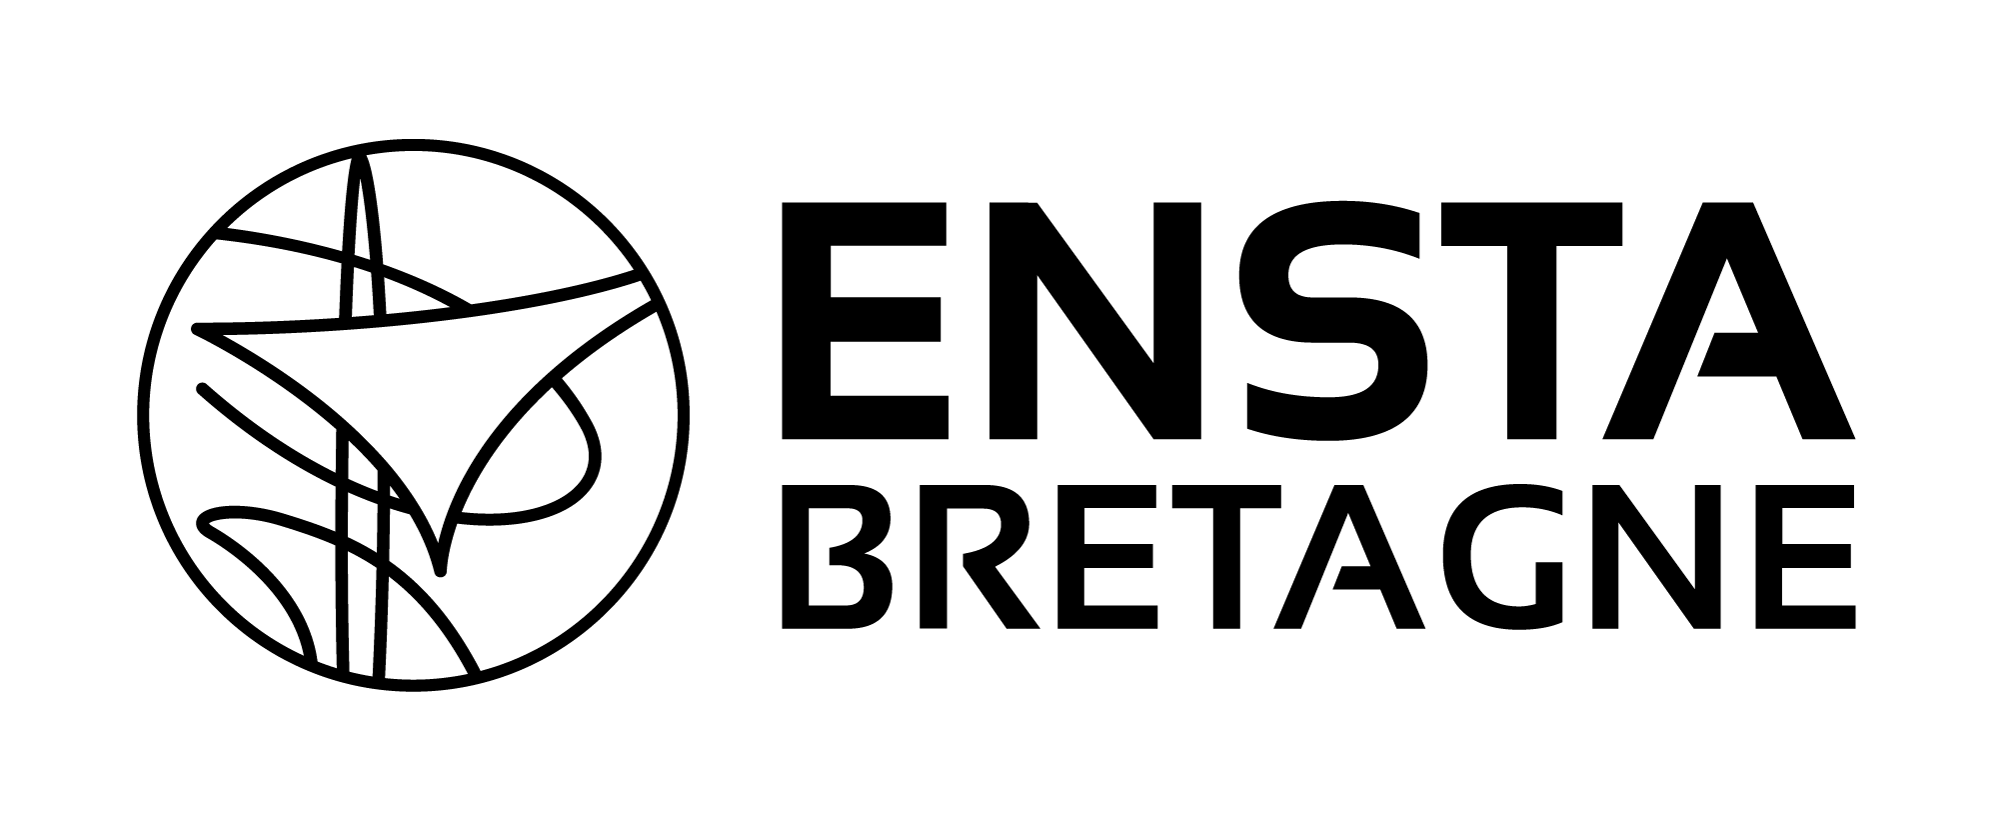
\includegraphics[width=0.8\textwidth]{ensta-logo-noir.png}\\[1cm]
\end{center}

% ---------- Titre principal ----------
\begin{center}
    {\Huge \bfseries \color{black}
    Rapport \\
    projet info}\\[0.7cm]
\end{center}

\vfill

% ---------- Auteurs ----------
\begin{center}
    {\large \bfseries \color{black}
    Victor CACHAU, \\ Xavier CAPDEVILLE}
\end{center}


\vfill

% ---------- Promo ----------
\begin{center}
    {\Large \bfseries \color{gray!60!black!85}
   FISE 2028}\\[1.75cm]
\end{center}

\vspace{0.5cm}

% ---------- Date ----------
\begin{center}
    {\large \color{black}
    % DATE DE SOUMISSION / RÉDACTION
    \today}
\end{center}


\end{titlepage}

% ------------------------------------------------------------------------------


\thispagestyle{empty}

\newpage
\tableofcontents
\thispagestyle{fancy}

\newpage


\section{Introduction}


Ce rapport présente le projet informatique réalisé dans le cadre de l'UE 2.1 à l'ENSTA Bretagne.
L'objectif est de concevoir et d'implémenter un jeu de stratégie de type 4X (\textit{eXplore,
eXpand, eXploit, eXterminate}) en Python, jouable au tour par tour avec une interface
graphique.

Le projet, baptisé \textbf{Imperium Novum }, modélise un monde procédural sur lequel un joueur
déplace des unités, fonde des villes, exploite des ressources et entre en conflit avec des
adversaires. L'implémentation s'appuie sur la bibliothèque \texttt{pygame} pour le rendu
graphique et \texttt{scipy} pour la génération procédurale de la carte.

L'architecture repose sur un système de \textbf{royaumes} (\texttt{Kingdom}) : chaque acteur du
jeu (joueur humain ou intelligence artificielle) est encapsulé dans un royaume identifié,
ce qui prépare un support multi-IA extensible. Un cadre abstrait (\texttt{BaseAI}) est déjà en
place ; les contrôleurs d'IA concrets se branchent sur ce cadre via un cycle de tour
Joueur\,$\to$\,IA\,$\to$\,Fin de tour.

\begin{figure}[H]
  \centering
  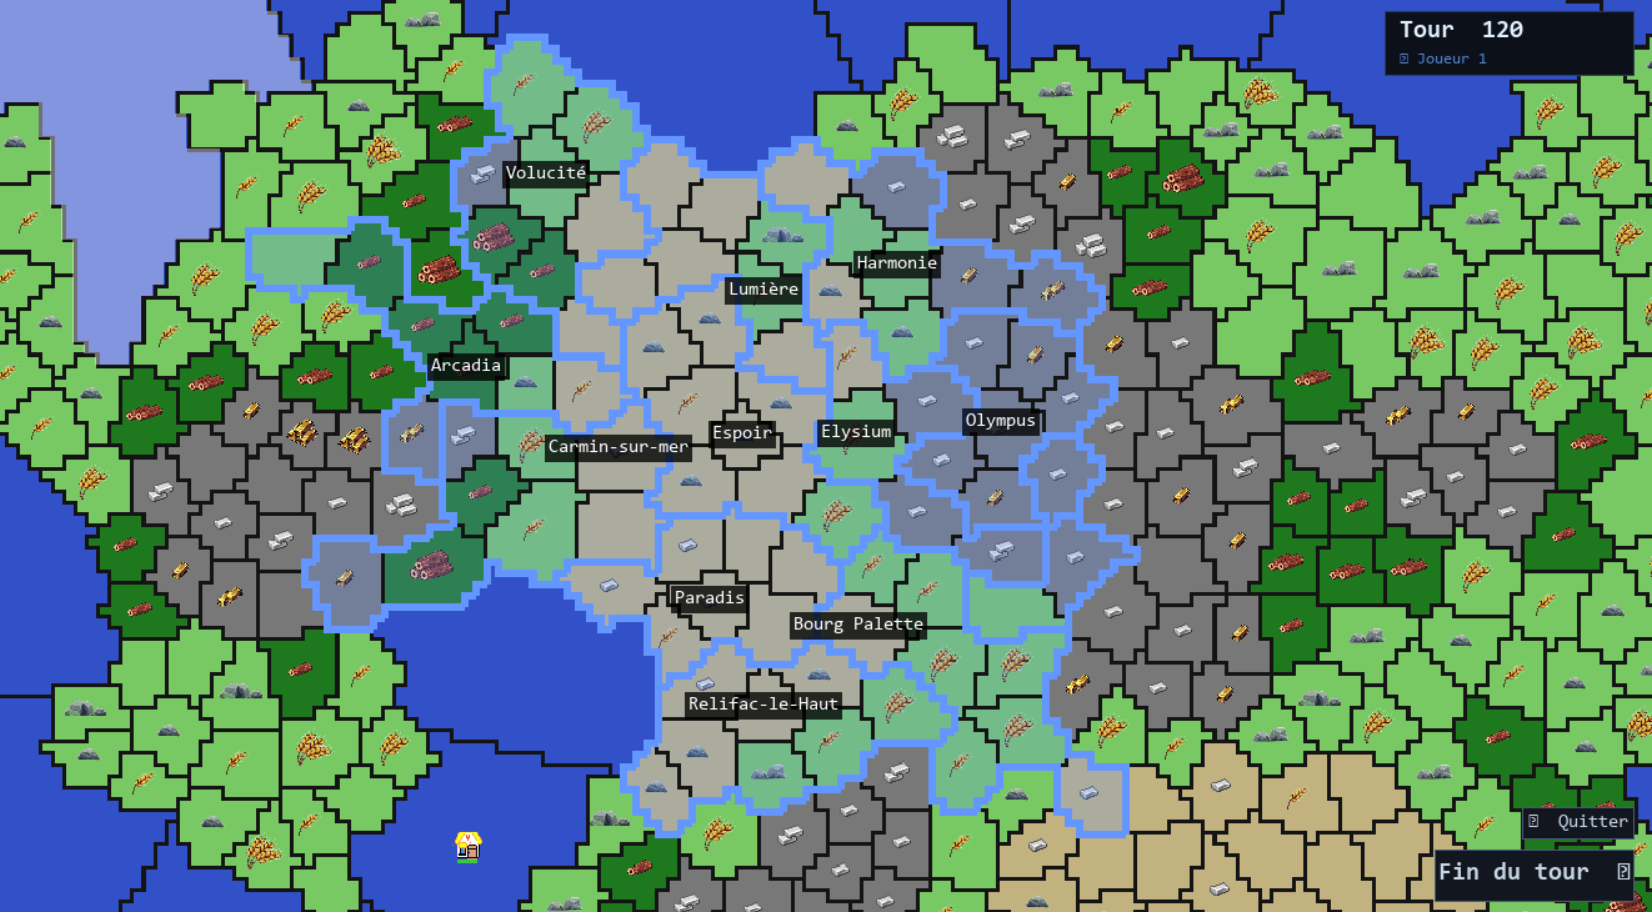
\includegraphics[width=0.85\textwidth]{../screenshots/villes.png}
  \caption{Interface générale de \textit{Imperium Novum } : carte procédurale avec villes, unités et indicateur de tour (tour 120)}
  \label{fig:ihm_general}
\end{figure}

Il convient de noter que les visuels intégrés à ce stade du projet sont des éléments de substitution (placeholders). N'ayant pas vocation à nous substituer à des professionnels du graphisme, nous nous sommes concentrés sur l'aspect fonctionnel et structurel de l'interface, laissant la charte graphique finale à la discrétion d'experts métier.


\section{Analyse du problème}


\subsection{Définition exacte du problème}

Un jeu 4X est un genre de jeu de stratégie dans lequel chaque joueur développe une
civilisation selon quatre axes fondamentaux :
\begin{enumerate}
    \item \textbf{eXploration} : découvrir la carte progressivement à travers un brouillard de guerre ;
    \item \textbf{eXpansion} : fonder des villes et étendre leur territoire ;
    \item \textbf{eXploitation} : collecter des ressources et construire des bâtiments ;
    \item \textbf{eXtermination} : attaquer les unités et villes adverses.
\end{enumerate}

Le problème consiste à modéliser informatiquement ces quatre mécaniques de façon cohérente,
dans un système tour par tour. La carte est une grille de provinces (\textit{tuiles}) de types
variés, chacune pouvant contenir des unités et des ressources. Plusieurs systèmes interagissent
simultanément : la gestion du mouvement, du combat, de l'économie et de la visibilité.

\subsection{Buts du projet}

Les objectifs définis pour ce projet sont les suivants :
\begin{itemize}
    \item Concevoir une architecture orientée objet claire et modulaire ;
    \item Générer procéduralement une carte de jeu variée et jouable ;
    \item Implémenter les mécaniques fondamentales : déplacement, combat, production, exploration ;
    \item Réaliser une interface graphique interactive permettant de jouer effectivement une
    partie ;
    \item Respecter des règles de jeu équilibrées (coûts de terrain, triangles d'efficacité
    des unités, expansion des villes) ;
    \item Fournir une architecture permettant l'ajout d'IA ennemies.
\end{itemize}

\subsection{Domaines d'utilisation}

Ce projet relève de plusieurs domaines informatiques :

\begin{description}
    \item[Algorithmique de graphes] : pathfinding avec Dijkstra sur un graphe de provinces,
    BFS pour la visibilité et l'expansion des villes, transformée de distance pour la
    génération de super-tuiles d'eau.
    \item[Génération procédurale] : bruit de Perlin multi-octaves pour les biomes, échantillonnage
    de Poisson pour les centres de provinces, diagrammes de Voronoï pour la partition de la carte.
    \item[Programmation orientée objet] : hiérarchie de classes (unités, villes, constructions,
    royaumes), patron Facade pour le moteur de jeu, pattern Factory pour les unités, classe
    abstraite \texttt{BaseAI} pour les contrôleurs IA.
    \item[Infographie 2D] : rendu Pygame avec surfaces mises en cache par couches, système de
    caméra avec zoom et panoramique, interface utilisateur (barres, menus contextuels
    multi-catégories).
\end{description}

% \subsection{Limites actuelles du projet}

% Plusieurs limites sont actuellement dans le projet et seront adressées dans les versions futures :
% \begin{itemize}

%     \item \textbf{Statistiques d'unités en cours d'équilibrage} : les statistiques des unités et de
%     production des villes sont des valeurs temporaires, un équilibrage est nécessaire pour que le jeu soit réellement jouable.

%     \item \textbf{Absence de condition de victoire} : aucune condition de fin de partie n'est
%     formalisée dans le code (pas de score, pas de domination, pas de limite de tours).

%     \item \textbf{Dépendance à la résolution} : la carte est définie en 444$\times$250 tuiles
%     avec une taille de tuile de 2 pixels, limitant la résolution effective à 888$\times$500
%     pixels avant zoom.
% \end{itemize}


\section{Description des classes}

La figure~\ref{fig:diagramme_classes} présente le diagramme de classes UML complet du projet. La figure~\ref{fig:uml_packages} en donne une vue détaillée par package.

\begin{figure}[H]
  \centering
  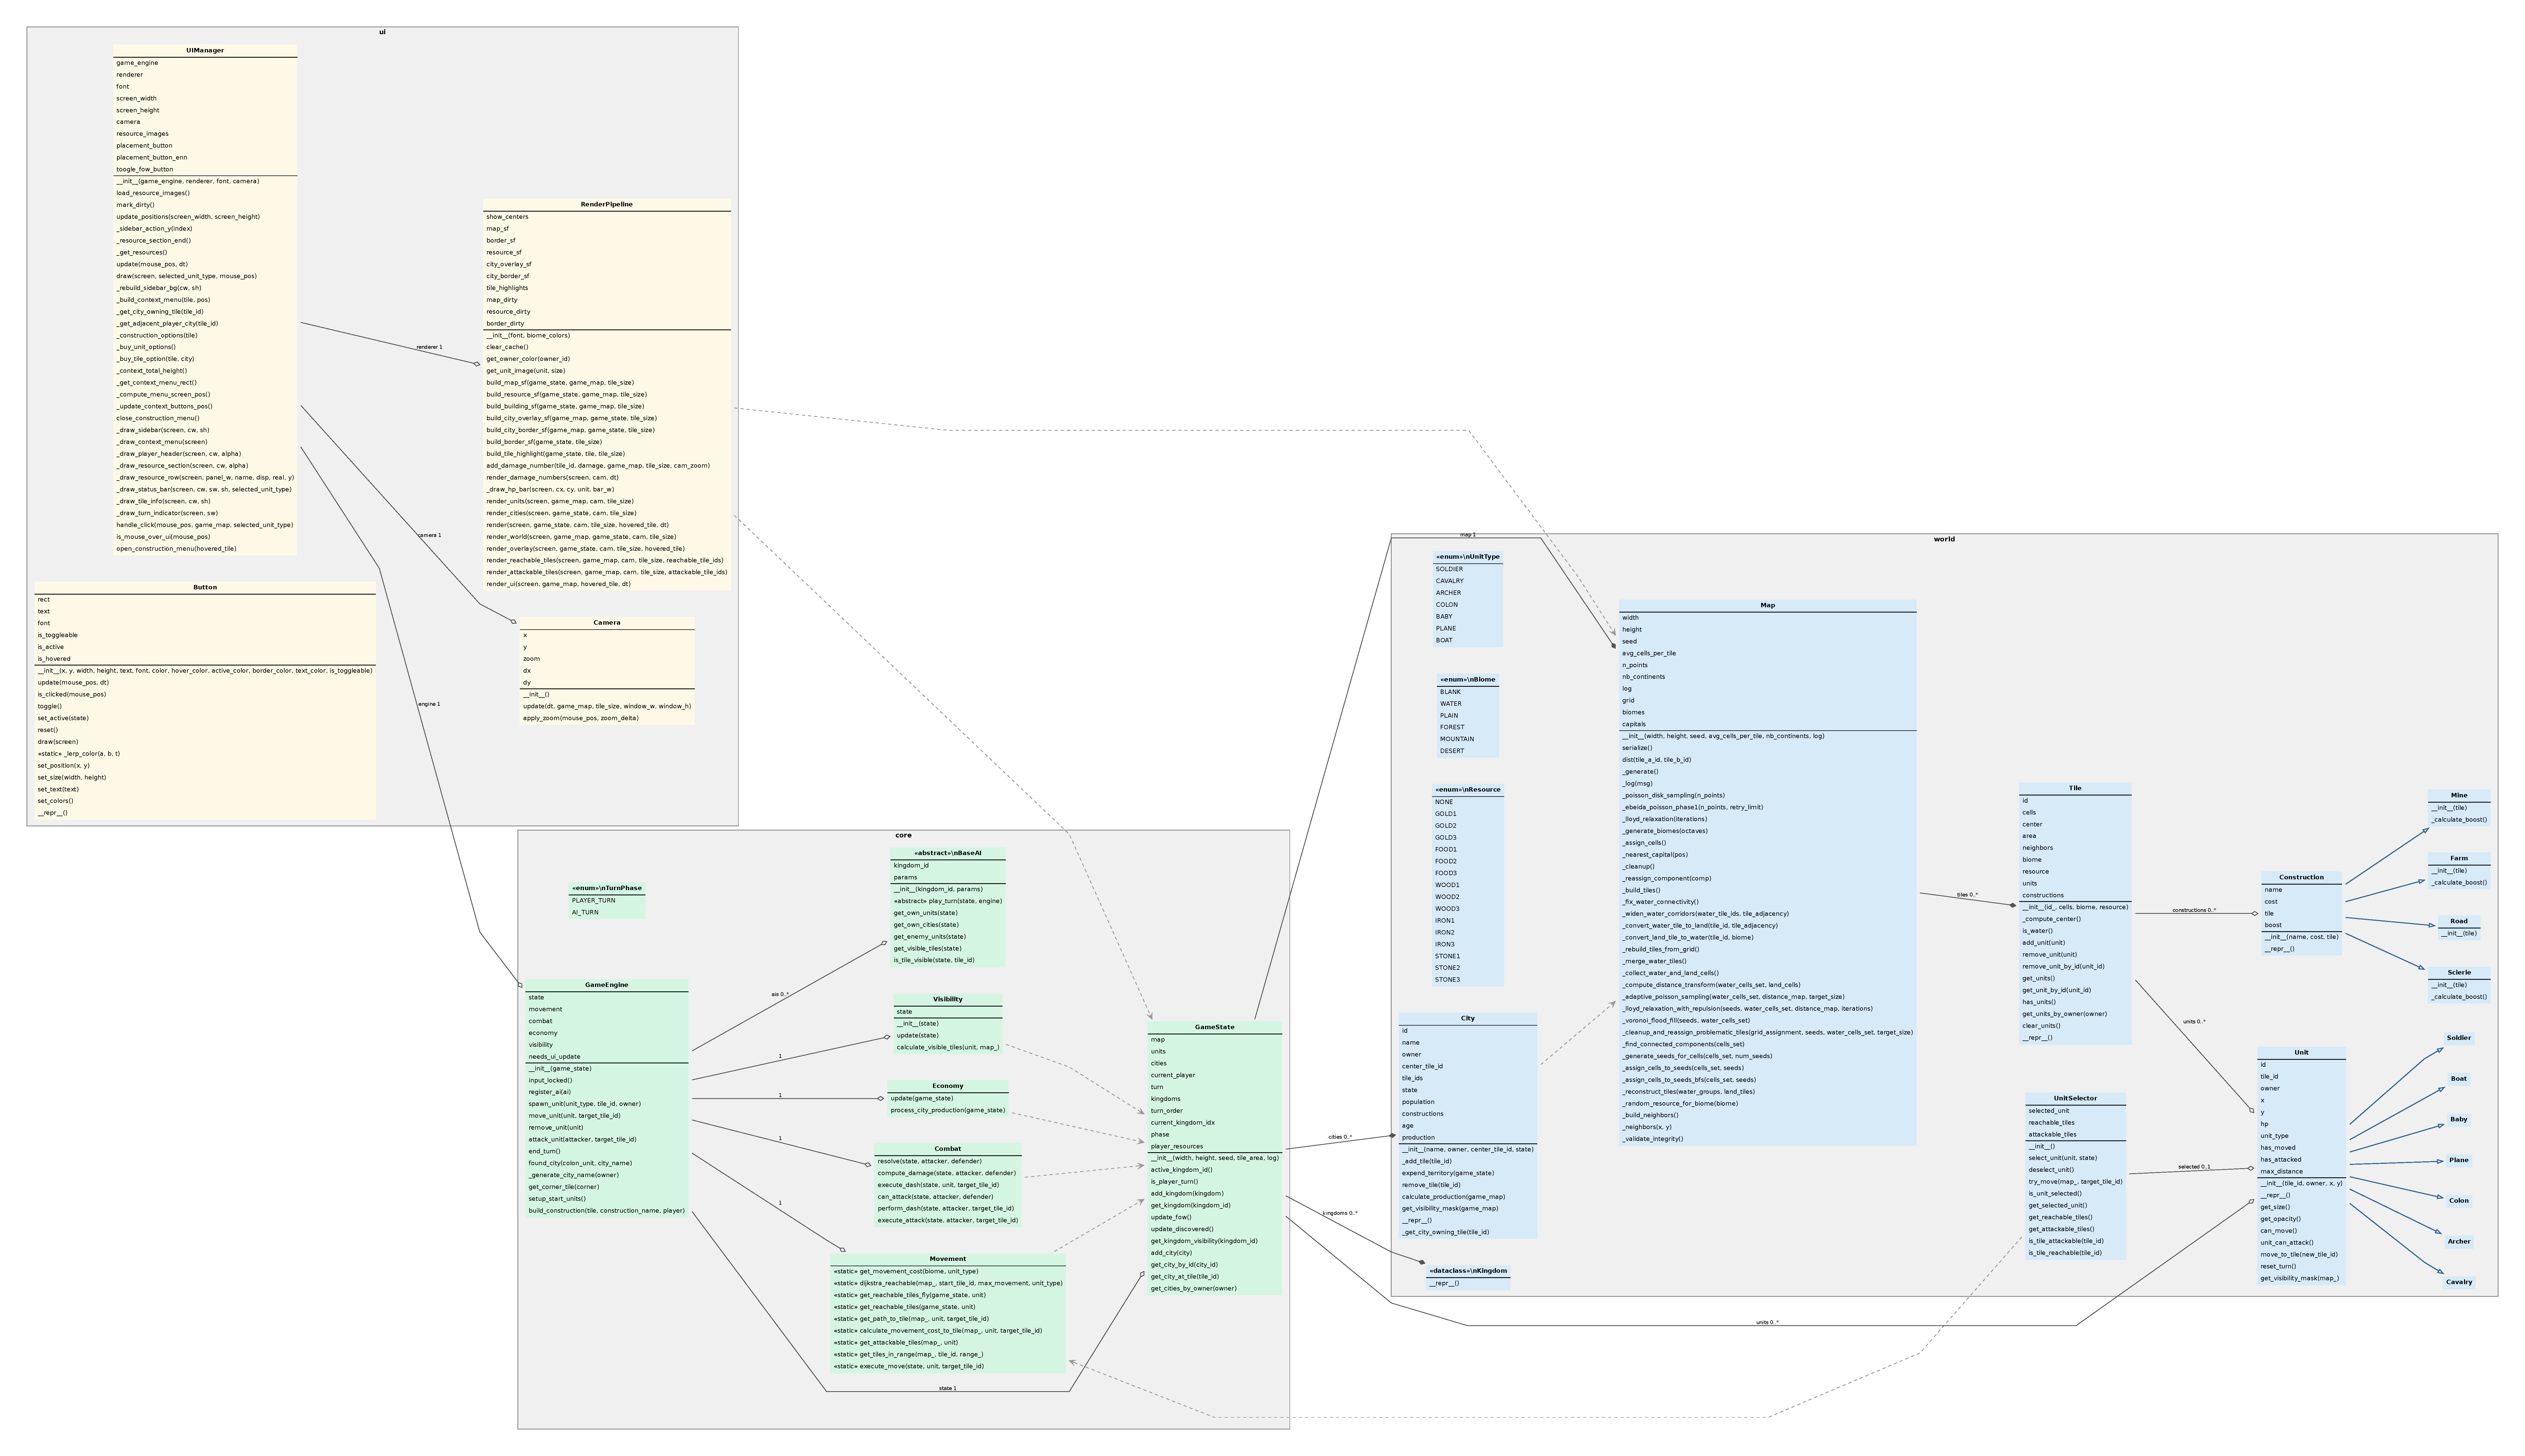
\includegraphics[width=\textwidth, height=0.88\textheight, keepaspectratio]{uml_classes.pdf}
  \caption{Diagramme de classes UML complet de \textit{Imperium Novum} (généré par graphviz)}
  \label{fig:diagramme_classes}
\end{figure}

\begin{figure}[H]
  \centering
  \begin{subfigure}{\textwidth}
    \centering
    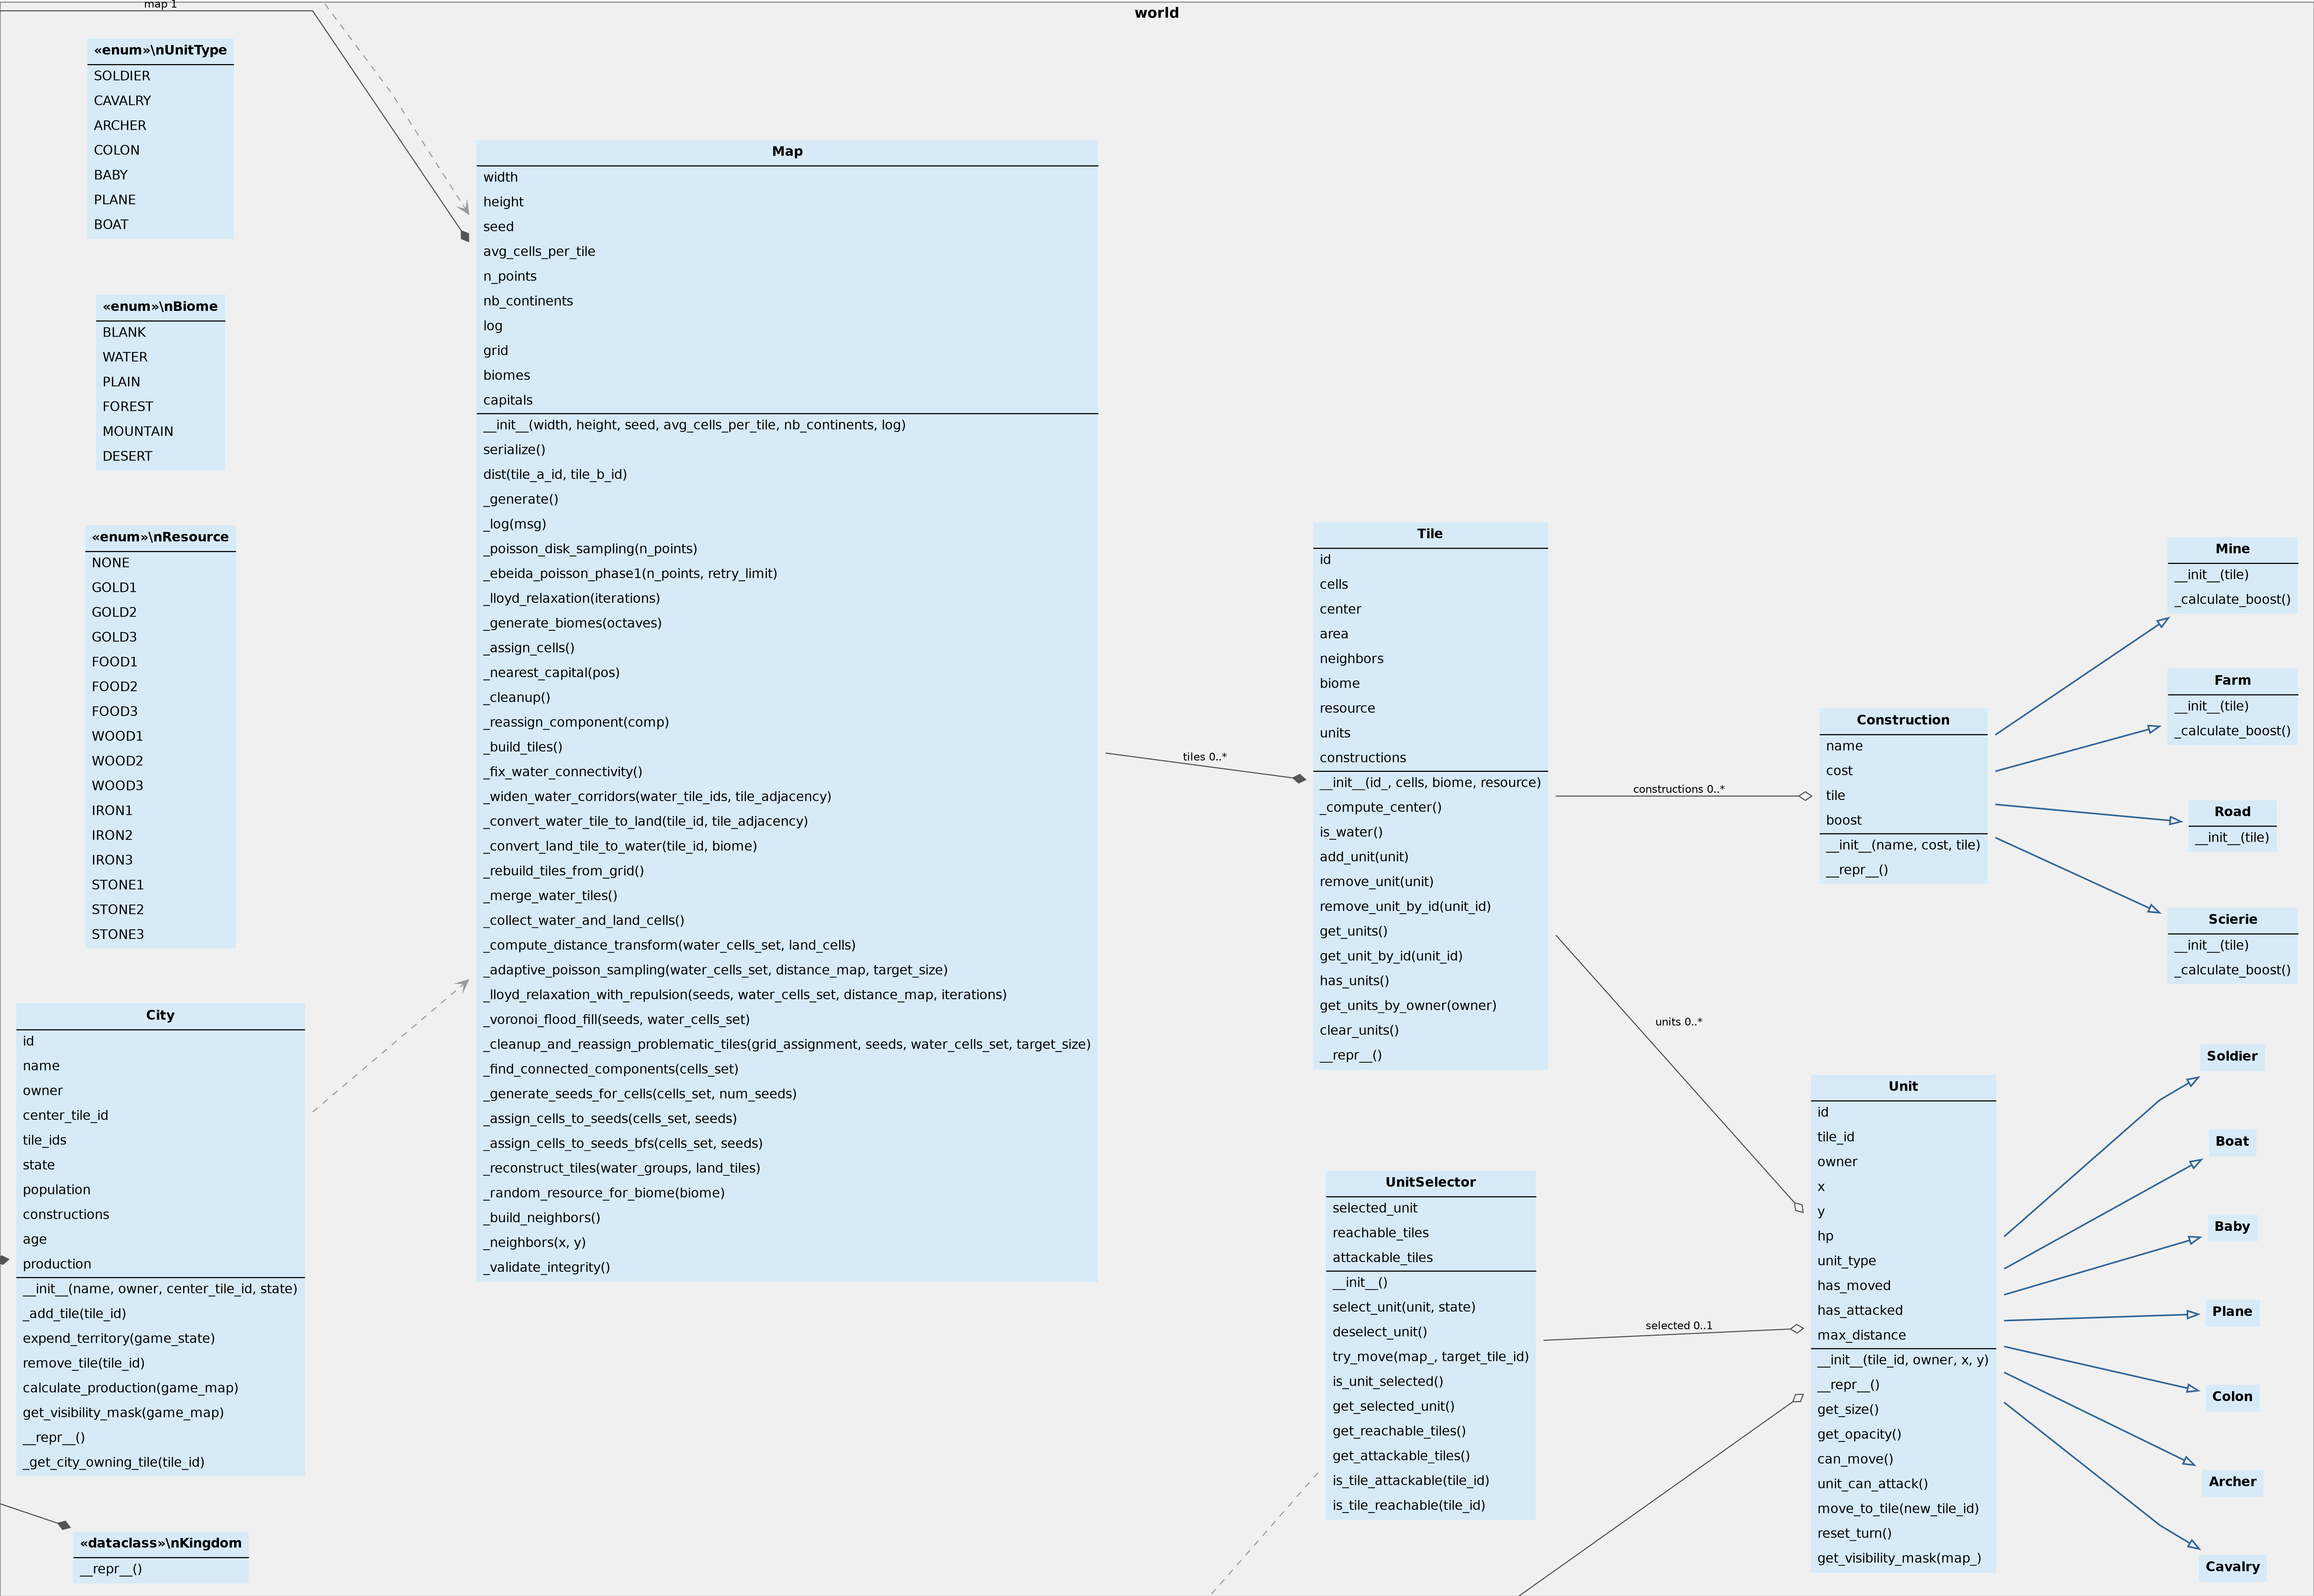
\includegraphics[width=\textwidth, height=0.30\textheight, keepaspectratio]{uml_world.png}
    \caption{Package \texttt{world} — modèle du jeu (unités, tuiles, carte, villes, constructions)}
    \label{fig:uml_world}
  \end{subfigure}

  \vspace{0.5em}

  \begin{subfigure}{\textwidth}
    \centering
    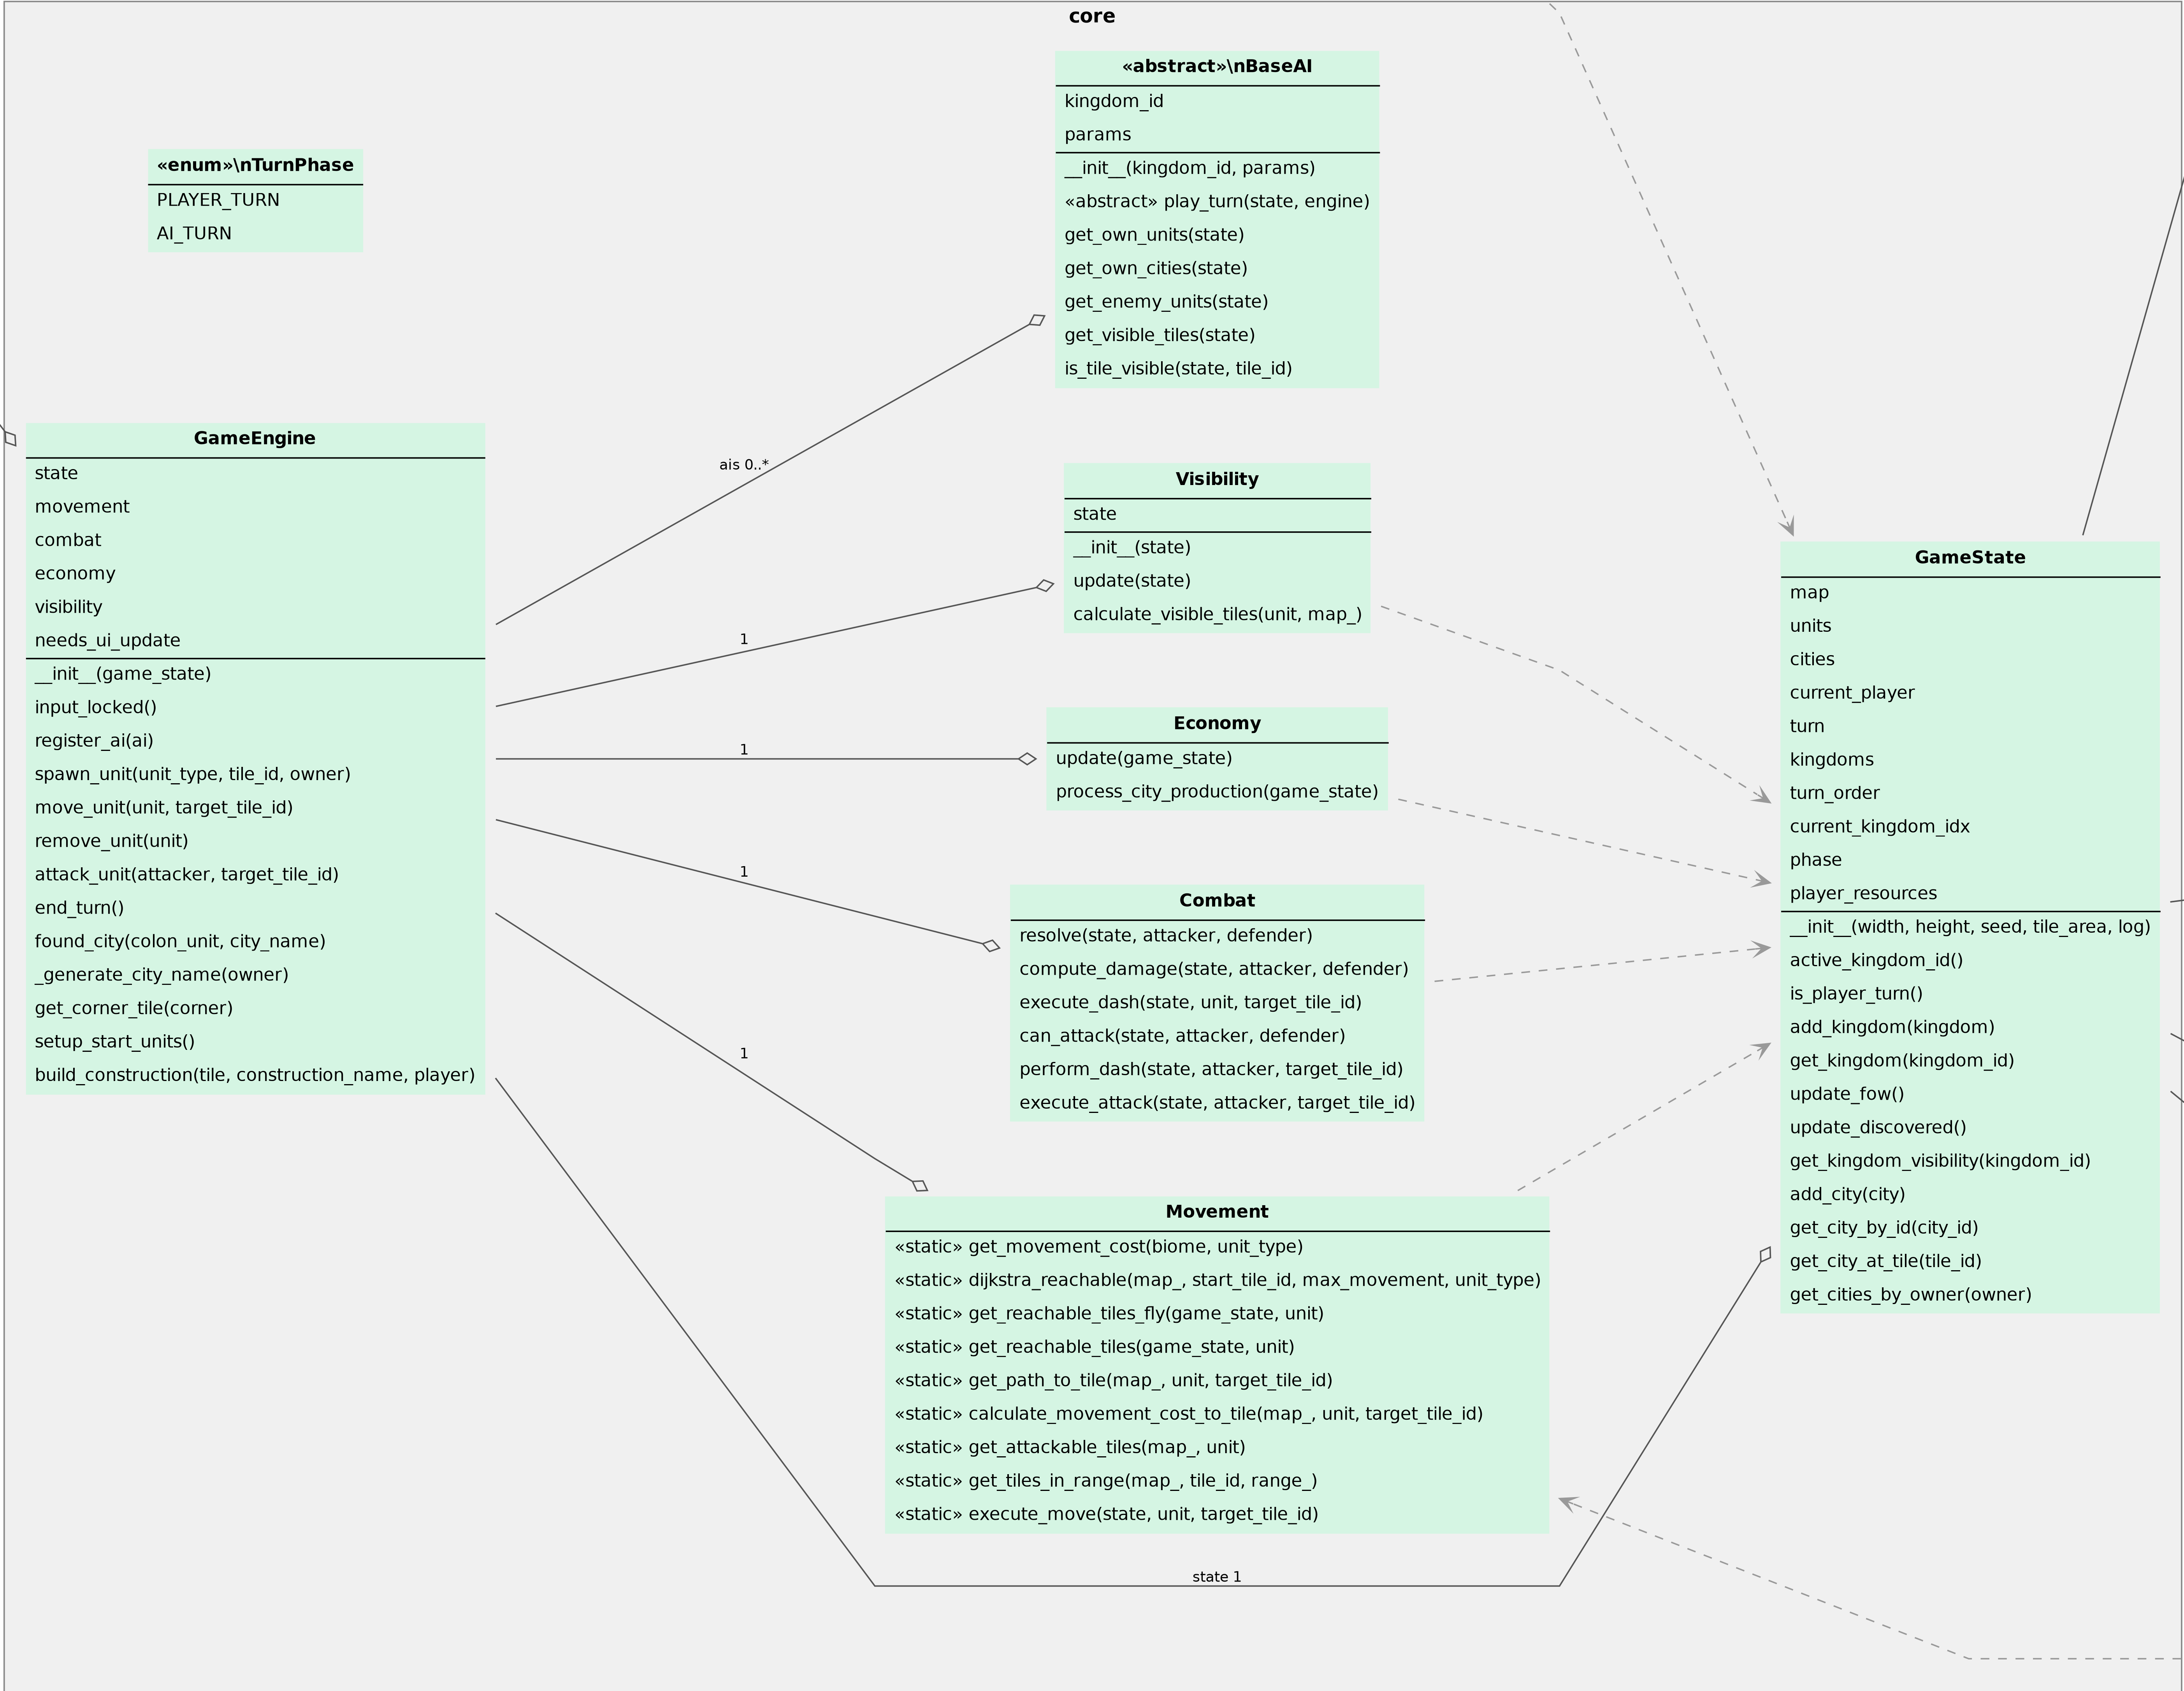
\includegraphics[width=\textwidth, height=0.30\textheight, keepaspectratio]{uml_core.png}
    \caption{Package \texttt{core} — moteur, état global et systèmes (combat, mouvement, économie, visibilité)}
    \label{fig:uml_core}
  \end{subfigure}

  \vspace{0.5em}

  \begin{subfigure}{\textwidth}
    \centering
    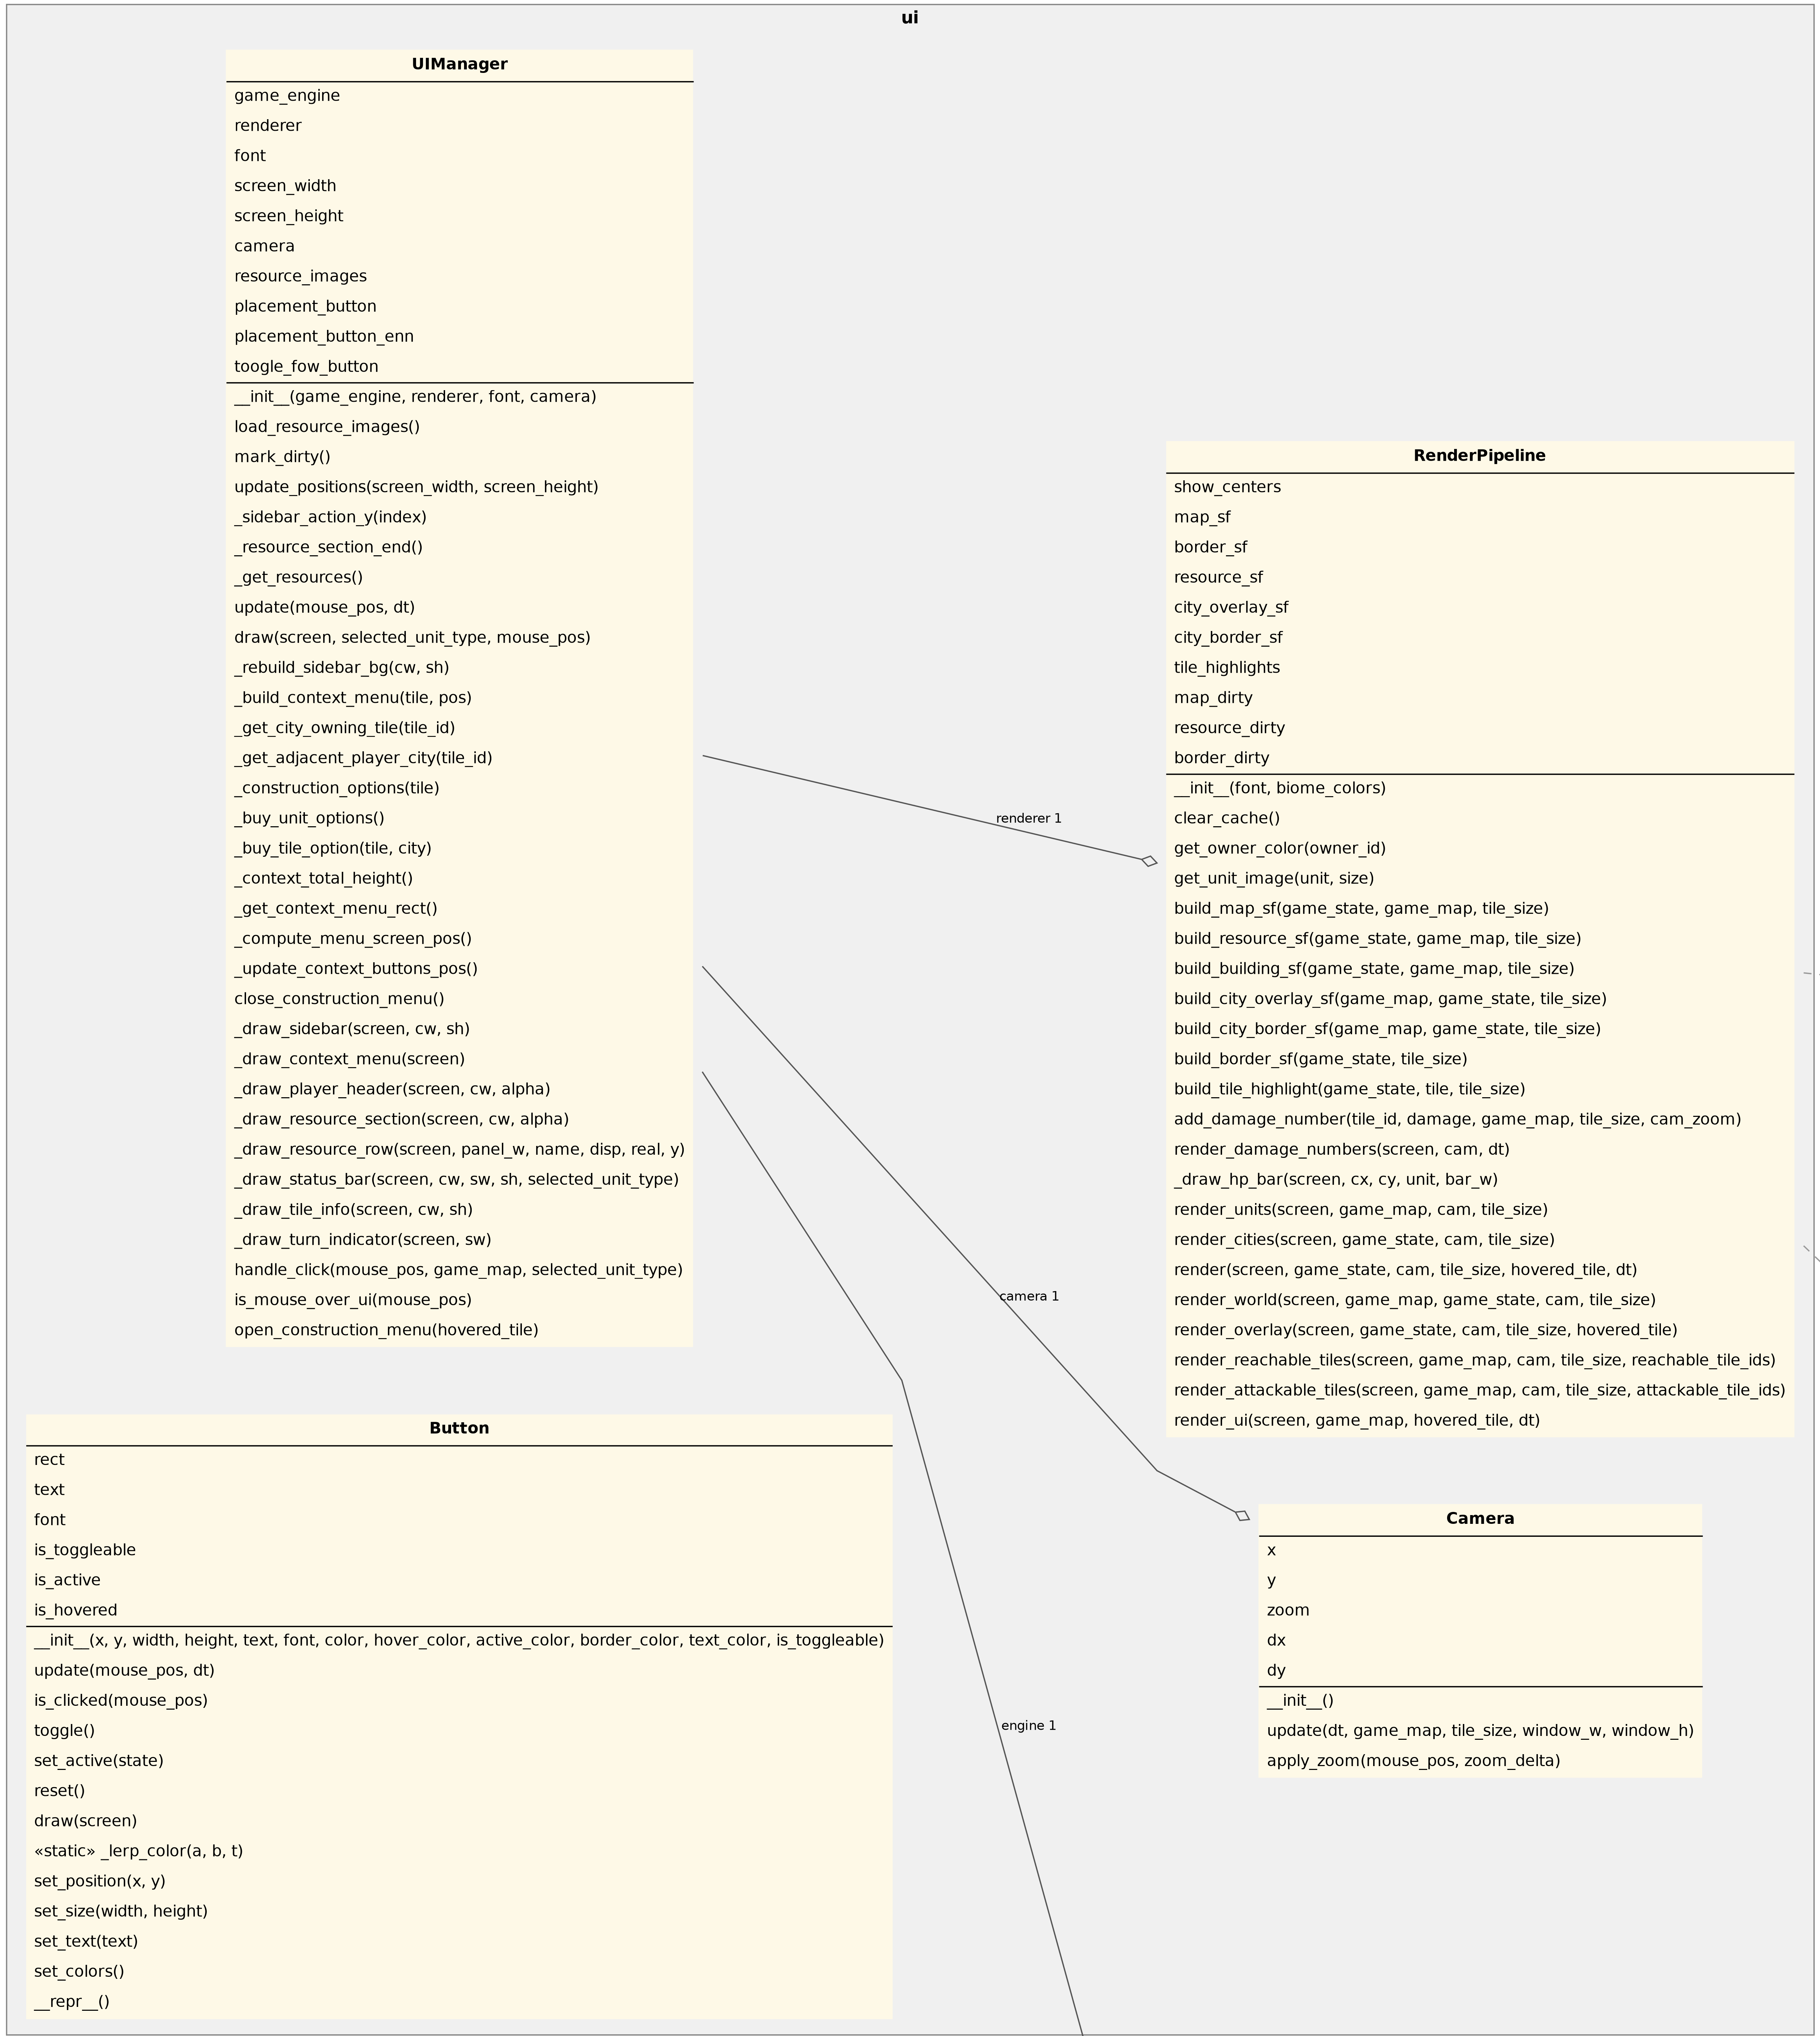
\includegraphics[width=\textwidth, height=0.25\textheight, keepaspectratio]{uml_ui.png}
    \caption{Package \texttt{ui} — interface graphique (gestionnaire UI, rendu, caméra, boutons)}
    \label{fig:uml_ui}
  \end{subfigure}

  \caption{Diagrammes UML détaillés par package}
  \label{fig:uml_packages}
\end{figure}

Le tableau suivant résume l'organisation modulaire du projet :

\begin{figure}[H]
    \begin{center}
    \begin{tabular}{ll}
    \toprule
    \textbf{Module} & \textbf{Rôle} \\
    \midrule
    \texttt{run\_project.py} & Point d'entrée (délègue à \texttt{ui/main.py}) \\
    \texttt{config.py} & Constantes globales de configuration \\
    \texttt{core/} & Moteur du jeu \\
    \texttt{\phantom{core}game\_state.py} & État global du jeu + phases de tour \\
    \texttt{\phantom{core}game\_engine.py} & Orchestrateur (façade) \\
    \texttt{\phantom{core}systems/} & Systèmes fondamentaux \\
    \texttt{\phantom{coresystems}movement.py} & Système de déplacement \\
    \texttt{\phantom{coresystems}combat.py} & Système de combat \\
    \texttt{\phantom{coresystems}economy.py} & Système économique \\
    \texttt{\phantom{coresystems}visibility.py} & Brouillard de guerre \\
    \texttt{\phantom{core}ai/base\_ai.py} & Interface abstraite des contrôleurs IA \\
    \texttt{world/} & Génération et stockage de la carte \\
    \texttt{\phantom{world}map.py} & Génération et stockage de la carte \\
    \texttt{\phantom{world}tile.py} & Province individuelle \\
    \texttt{\phantom{world}unit.py} & Hiérarchie des unités + factory \\
    \texttt{\phantom{world}city.py} & Gestion des villes \\
    \texttt{\phantom{world}kingdom.py} & Représentation d'un royaume (joueur ou IA) \\
    \texttt{\phantom{world}construction.py} & Bâtiments (Ferme, Mine, Route, Scierie) \\
    \texttt{\phantom{world}resources.py} & Enumération des types de ressources \\
    \texttt{\phantom{world}biome.py} & Enumération des biomes \\
    \texttt{\phantom{world}selector.py} & Sélection d'unité, zones accessibles/attaquables \\
    \texttt{ui/} & Logique du rendu graphique \\
    \texttt{\phantom{ui}main.py} & Boucle principale du jeu \\
    \texttt{\phantom{ui}renderer.py} & Pipeline de rendu Pygame \\
    \texttt{\phantom{ui}camera.py} & Caméra avec zoom et panoramique \\
    \texttt{\phantom{ui}ui\_manager.py} & Gestionnaire de l'interface utilisateur \\
    \texttt{utils/noise.py} & Bruit de Perlin \\
    \bottomrule
    \end{tabular}
    \end{center}
    \caption{Tableau récapitulatif des modules et de leurs rôles dans le projet}
    \label{fig:tableau_modules}
\end{figure}

\subsection{GameConfig (config.py)}

\textit{GameConfig} est une classe de configuration regroupant toutes les constantes du jeu sous forme d'attributs de
classe. Elle évite la dispersion des paramètres dans le code et centralise les réglages de la
carte, des boutons, de l'interface et des villes.

\begin{lstlisting}[
    style=python,
    caption={Extrait de \texttt{config.py}}, label={lst:config_extract}
    ]
class GameConfig:
    TILE_SIZE = 2
    TILE_AVG_AREA = 35          # Taille moyenne d'une province (en cellules)
    HEIGHT = 250                # Hauteur de la carte en tuiles
    WIDTH = (HEIGHT * 16) // 9  # Largeur 16:9
    CITY_MIN_TURN_EXTENTION_AVAILABLE = [3, 5, 8, 13, 21, 34, 53, 89]
    CITY_EXTENSION_RADIUS = 3
    SIDEBAR_WIDTH = 210
    STATUS_H = 52
\end{lstlisting}

\subsection{Kingdom (world/kingdom.py)}

\textit{Kingdom} est une dataclass représentant un royaume, qu'il soit contrôlé par un joueur humain ou par une IA.
Chaque royaume possède une identité visuelle (couleur RGB) et, s'il est IA, un dictionnaire
\texttt{ai\_params} calibrant son arbre de décision.

Attributs :
\begin{itemize}
    \item \texttt{kingdom\_id} : identifiant unique (0 = joueur humain) ;
    \item \texttt{name} : nom du royaume (ex. \og Joueur 1 \fg{}, \og Barbares \fg{}) ;
    \item \texttt{color} : tuple RGB utilisé pour la couleur d'affichage UI ;
    \item \texttt{is\_ai} : \texttt{True} si le royaume est contrôlé par une IA ;
    \item \texttt{ai\_params} : paramètres de décision (\texttt{aggression}, \texttt{exploration},
    \texttt{expansion}, \texttt{defense}).
\end{itemize}

\subsection{TurnPhase (core/game\_state.py)}

Enumération à deux valeurs gérant la phase active dans le cycle de tour :
\begin{itemize}
    \item \texttt{PLAYER\_TURN} : le joueur humain peut interagir ;
    \item \texttt{AI\_TURN} : une IA est en cours de jeu, les entrées joueur sont verrouillées.
\end{itemize}

\subsection{GameState (core/game\_state.py)}

Classe centrale qui encapsule l'intégralité de l'état d'une partie en cours. Elle ne contient
pas de logique métier, mais sert de structure de données partagée entre tous les systèmes.

Attributs principaux :
\begin{itemize}
    \item \texttt{map} : l'objet \texttt{Map} généré procéduralement ;
    \item \texttt{units} : liste de toutes les unités en jeu ;
    \item \texttt{cities} : liste de toutes les villes fondées ;
    \item \texttt{kingdoms} : liste des objets \texttt{Kingdom} enregistrés ;
    \item \texttt{turn\_order} : liste ordonnée des \texttt{kingdom\_id} dans l'ordre de jeu ;
    \item \texttt{current\_kingdom\_idx} : index courant dans \texttt{turn\_order} (utilisé pendant la phase IA) ;
    \item \texttt{phase} : valeur de \texttt{TurnPhase} indiquant la phase active ;
    \item \texttt{player\_resources} : dictionnaire \texttt{\{kingdom\_id: \{ressource: quantité\}\}} ;
    \item \texttt{turn} : compteur de tours ;
    \item \texttt{discovered}, \texttt{visibility} : bitmasks pour le brouillard de guerre ;
    \item \texttt{use\_ti}, \texttt{use\_fow} : drapeaux pour activer la \textit{terra incognita} et
    le brouillard de guerre.
\end{itemize}

Propriétés calculées :
\begin{itemize}
    \item \texttt{active\_kingdom\_id} : ID du royaume dont c'est actuellement le tour ;
    \item \texttt{is\_player\_turn} : \texttt{True} si le joueur humain peut agir.
\end{itemize}

\subsection{GameEngine (core/game\_engine.py)}

Moteur de jeu central qui implémente un patron \textit{Facade} : il délègue chaque action à
un système spécialisé tout en gérant les effets de bord (mise à jour de la visibilité, retrait
des unités mortes, incrémentation des tours).

Systèmes délégués :
\begin{itemize}
    \item \texttt{self.movement} : classe statique \texttt{Movement} ;
    \item \texttt{self.combat} : instance de \texttt{Combat} ;
    \item \texttt{self.economy} : instance de \texttt{Economy} ;
    \item \texttt{self.visibility} : instance de \texttt{Visibility}.
\end{itemize}

Principales méthodes publiques :
\begin{itemize}
    \item \texttt{register\_ai(ai)} : associe un contrôleur \texttt{BaseAI} à un royaume IA ;
    \item \texttt{spawn\_unit(unit\_type, tile\_id, owner)} : instancie et place une unité ;
    \item \texttt{remove\_unit(unit)} : retire une unité du jeu et met à jour la visibilité ;
    \item \texttt{move\_unit(unit, target\_tile\_id)} : déplace une unité via \texttt{Movement} ;
    \item \texttt{attack\_unit(attacker, target\_tile\_id)} : résout un combat via \texttt{Combat} ;
    \item \texttt{found\_city(colon, city\_name)} : fonde une ville à l'emplacement d'un colon ;
    \item \texttt{build\_construction(tile, name, player)} : construit un bâtiment sur une tuile ;
    \item \texttt{setup\_start\_units()} : place le colon initial de chaque royaume dans un coin de la carte ;
    \item \texttt{end\_turn()} : clôture le tour du joueur et déclenche les tours IA.
\end{itemize}

La propriété \texttt{input\_locked} retourne \texttt{True} pendant \texttt{AI\_TURN},
ce qui permet à la boucle principale de bloquer toutes les entrées joueur le temps que
les IA jouent.

\subsection{BaseAI (core/ai/base\_ai.py)}

Classe abstraite (ABC) définissant l'interface que doit respecter tout contrôleur IA.

\begin{lstlisting}[style=python, caption={Interface abstraite \texttt{BaseAI}}]
class BaseAI(ABC):
    def __init__(self, kingdom_id: int, params: dict): ...

    @abstractmethod
    def play_turn(self, state: GameState, engine: GameEngine) -> None:
        """Appele une fois par tour ; doit utiliser engine.move_unit()
        et engine.attack_unit() -- ne modifie pas state directement."""
        ...

    # Helpers lecture seule :
    def get_own_units(self, state): ...
    def get_own_cities(self, state): ...
    def get_enemy_units(self, state): ...
    def get_visible_tiles(self, state) -> int: ...
    def is_tile_visible(self, state, tile_id) -> bool: ...
\end{lstlisting}

Pour ajouter une IA, il suffit de sous-classer \texttt{BaseAI}, d'implémenter
\texttt{play\_turn()}, puis d'appeler \texttt{engine.register\_ai(MonIA(kingdom\_id=1,
params=...))} avant la boucle de jeu.

\subsection{Unit et sous-classes (world/unit.py)}

\texttt{Unit} est une classe de base abstraite définissant l'interface commune à toutes les
unités. Elle ne doit pas être instanciée directement. Chaque sous-classe redéfinit les
attributs de classe (constantes) décrivant ses caractéristiques.

\medskip
\noindent\textbf{Capacités spéciales des unités :}
\begin{description}
    \item[\texttt{DASH}] : peut se déplacer et attaquer en un seul tour ;
    \item[\texttt{ESCAPE}] : peut se déplacer après avoir attaqué ;
    \item[\texttt{SCOUT}] : portée de visibilité étendue (2 couronnes de tuiles au lieu de 1);
    \item[\texttt{FLY}] : ignore les coûts de terrain (traverse eau, montagne, forêt sans pénalité) ;
    \item[\texttt{PERSIST}] : peut attaquer tant qu'il y a des ennemis à portée, même après avoir attaqué (contrairement à DASH qui ne peut attaquer qu'une fois) ;
    \item[\texttt{WATER\_AFFINITY}] : peut traverser et se poser sur des tuiles d'eau ;
    \item[\texttt{LAND\_AFFINITY}] : peut se déplacer sur des tuiles terrestres.
\end{description}

\medskip
Le tableau \ref{tab:unites} suivant récapitule les caractéristiques de chaque unité.

\begin{table}[H]
\centering
\begin{tabular}{lrrrrrcl}
\toprule
\textbf{Type} & \textbf{ATK} & \textbf{DEF} & \textbf{PV} & \textbf{Mvt} & \textbf{Portée} & \textbf{Coût} & \textbf{Capacités} \\
\midrule
Soldier  & 5 & 8   & 100 & 3  & 1 & 8 & --- \\
Cavalry  & 12       & 6   & 90  & 5  & 1 & 150  & DASH, ESCAPE \\
Archer   & 8        & 5   & 70  & 2  & 2 & 10   & SCOUT \\
Colon    & 2        & 3   & 50  & 1  & 0 & 15   & WATER\_AFFINITY \\
Plane    & 20       & 5   & 50  & 10 & 10 & 500  & FLY, SCOUT, WATER\_AFFINITY \\
Boat     & 5        & 3   & 50  & 3  & 1 & 100   & WATER\_AFFINITY \\
\bottomrule
\end{tabular}
\caption{Caractéristiques des unités}
\label{tab:unites}
\end{table}

Une factory \texttt{UNIT\_CLASS\_MAP} associe chaque valeur de l'énumération \texttt{UnitType}
à la classe concrète correspondante.

\subsection{UnitSelector (world/selector.py)}

Gestionnaire de la sélection d'unités dans l'UI. Calcule et mémorise lors de la sélection :
\begin{itemize}
    \item \texttt{reachable\_tiles} : tuiles accessibles au mouvement ce tour (affichées en bleu) ;
    \item \texttt{attackable\_tiles} : tuiles contenant des ennemis à portée d'attaque (affichées en rouge).
\end{itemize}

Ces ensembles sont recalculés à chaque sélection en appelant
\texttt{Movement.get\_reachable\_tiles()} et \texttt{Movement.get\_attackable\_tiles()}.

\begin{figure}[H]
  \centering
  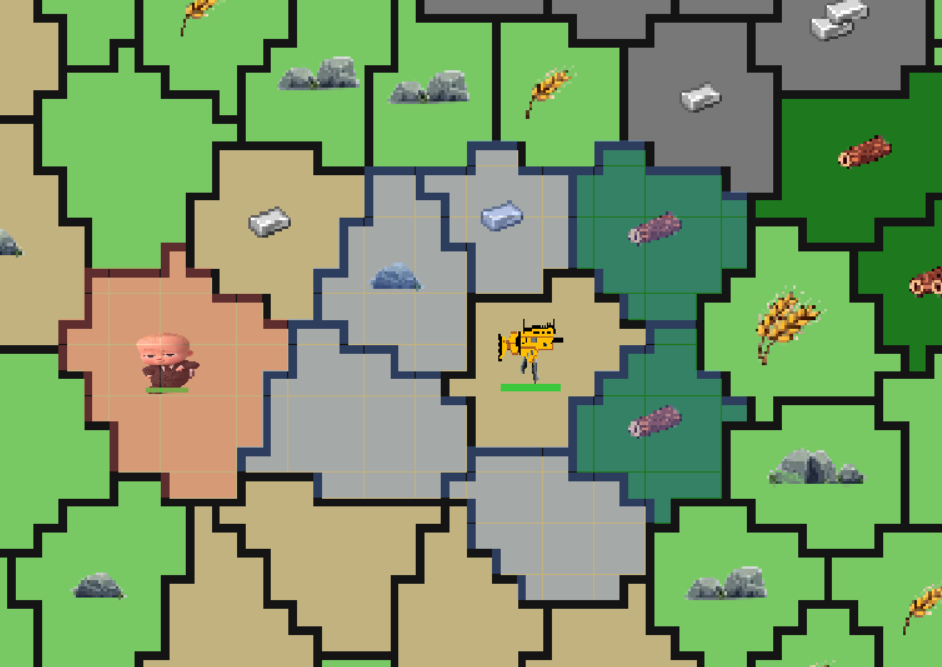
\includegraphics[width=0.85\textwidth]{../screenshots/portee_attaque.png}
  \caption{Visualisation des zones de mouvement (bleu) lors de la sélection d'un archer}
  \label{fig:unit_selection}
\end{figure}

\subsection{City (world/city.py)}

Représente une ville fondée par un colon. Une ville contrôle un ensemble de tuiles
(\texttt{tile\_ids}) et produit des ressources chaque tour en fonction des tuiles et des
bâtiments présents. L'expansion du territoire est déclenchée automatiquement à des âges
prédéfinis : $[3, 5, 8, 13, 21, 34, 53, 89]$ tours (suite de Fibonacci tronquée).

Attributs principaux :
\begin{itemize}
    \item \texttt{center\_tile\_id} : tuile fondatrice ;
    \item \texttt{tile\_ids} : territoire contrôlé (ensemble d'IDs de tuiles) ;
    \item \texttt{population}, \texttt{age} : état démographique et temporel ;
    \item \texttt{production} : dictionnaire \texttt{\{ressource: quantité/tour\}}.
\end{itemize}

La méthode \texttt{get\_visibility\_mask()} permet à une ville de contribuer à la visibilité
de son royaume : toutes les tuiles du territoire et leurs voisines immédiates sont visibles.

\subsection{Construction et sous-classes (world/construction.py)}

Quatre types de bâtiments peuvent être construits sur les tuiles contrôlées par une ville.
Le bonus de production est calculé dynamiquement à la construction en fonction de la ressource
présente sur la tuile.

\begin{table}[H]
\centering
\begin{tabular}{llll}
\toprule
\textbf{Bâtiment} & \textbf{Coût} & \textbf{Bonus calculé dynamiquement} \\
\midrule
Ferme     & 5 bois            & +1 à +3 nourriture (selon FOOD1/2/3 présente) \\
Mine      & 2 pierre + 3 bois & +1 à +3 fer/or/pierre selon ressource minière \\
Route     & 1 pierre + 1 bois & +1 mouvement sur la tuile \\
Scierie   & 5 bois            & +1 à +3 bois (selon WOOD1/2/3 présente) \\
\bottomrule
\end{tabular}
\caption{Constructions disponibles et effets sur la production}
\label{tab:constructions_inline}
\end{table}

La règle de placement autorise une route et un bâtiment non-route par tuile, mais pas deux
bâtiments non-route. Les routes peuvent coexister avec n'importe quel autre bâtiment.

\subsection{Map (world/map.py)}

Classe centrale de la carte. Elle stocke le dictionnaire \texttt{tiles:\{id: Tile\}} et
encapsule le pipeline de génération procédurale en sept étapes principales
(voir section~\ref{sec:methodes}). Elle utilise une structure de graphe par liste d'adjacence pour
permettre le pathfinding et la diffusion. La génération est entièrement pilotée par une
\texttt{seed} unique garantissant le déterminisme.

\subsection{Tile (world/tile.py)}

Représente une province individuelle. Chaque tuile possède :
\begin{itemize}
    \item un identifiant unique \texttt{id} ;
    \item un biome (\texttt{Biome}) et une ressource (\texttt{Resource}) ;
    \item une liste de cellules visuelles (\texttt{cells}) qui la composent ;
    \item un ensemble de voisins (\texttt{neighbors}) pour le graphe ;
    \item une liste d'unités présentes (\texttt{units}) et de constructions (\texttt{constructions}).
\end{itemize}

\subsection{Systèmes de jeu}

\subsubsection{Movement (core/systems/movement.py)}
Classe statique gérant les déplacements. Utilise l'algorithme de Dijkstra sur le graphe de
voisinage des tuiles avec des coûts variables selon le biome et le type d'unité.
Fournit également \texttt{get\_attackable\_tiles()} calculant les tuiles ennemies à portée
d'attaque (y compris la portée $\geq 2$ des archers et avions).

\subsubsection{Combat (core/systems/combat.py)}
Gère la résolution des combats selon une formule intégrant l'attaque, la défense, un
modificateur de terrain et un modificateur de type d'unité (triangle d'efficacité).
Gère également la mécanique de \textit{dash} de la cavalerie : déplacement et attaque
en une seule action.

\subsubsection{Economy (core/systems/economy.py)}
Calcule la production des villes (en recalculant \texttt{calculate\_production()} à chaque
tour pour tenir compte des nouvelles constructions) et déduit les coûts d'entretien des
unités en or à chaque fin de tour pour tous les royaumes actifs.

\subsubsection{Visibility (core/systems/visibility.py)}
Met à jour les bitmasks de visibilité et de découverte à partir des positions des unités et
des villes du joueur courant. Les unités de type SCOUT étendent la visibilité à deux couronnes
de tuiles au lieu d'une.

\subsection{Interface utilisateur}

\begin{itemize}
    \item \textbf{Camera (ui/camera.py)} : gère le panoramique et le zoom (1$\times$ à 25$\times$) avec conversion de coordonnées monde/écran.
    \item \textbf{Renderer (ui/renderer.py)} : pipeline de rendu en couches (carte, ressources, bâtiments, unités, brouillard, interface). Les surfaces Pygame sont mises en cache et reconstruites uniquement si marquées comme \textit{dirty}. Affiche aussi les nombres de dégâts animés lors des attaques.
    \item \textbf{UIManager (ui/ui\_manager.py)} : gère la barre latérale gauche (ressources, boutons), la barre de statut basse, l'indicateur de tour animé, et les menus contextuels multi-catégories (Construction / Unités / Territoire).
\end{itemize}

\subsubsection{Menu contextuel multi-catégories}

Un clic droit sur une tuile ouvre un menu contextuel dont les catégories disponibles dépendent
du contexte :

\begin{description}
    \item[Construction (bleu)] : visible sur toute tuile terrestre (appartenant au joueur ou neutre) ;
    propose Ferme, Mine, Route, Scierie selon le biome et les constructions déjà présentes.
    \item[Unités (rouge)] : visible uniquement sur les tuiles appartenant à une ville du joueur ;
    permet d'acheter Soldat, Archer ou Colon en dépensant de l'or.
    \item[Territoire (or)] : visible sur les tuiles libres adjacentes à une ville du joueur ;
    permet d'annexer la tuile pour 10 pièces d'or.
\end{description}

\begin{figure}[H]
  \centering
  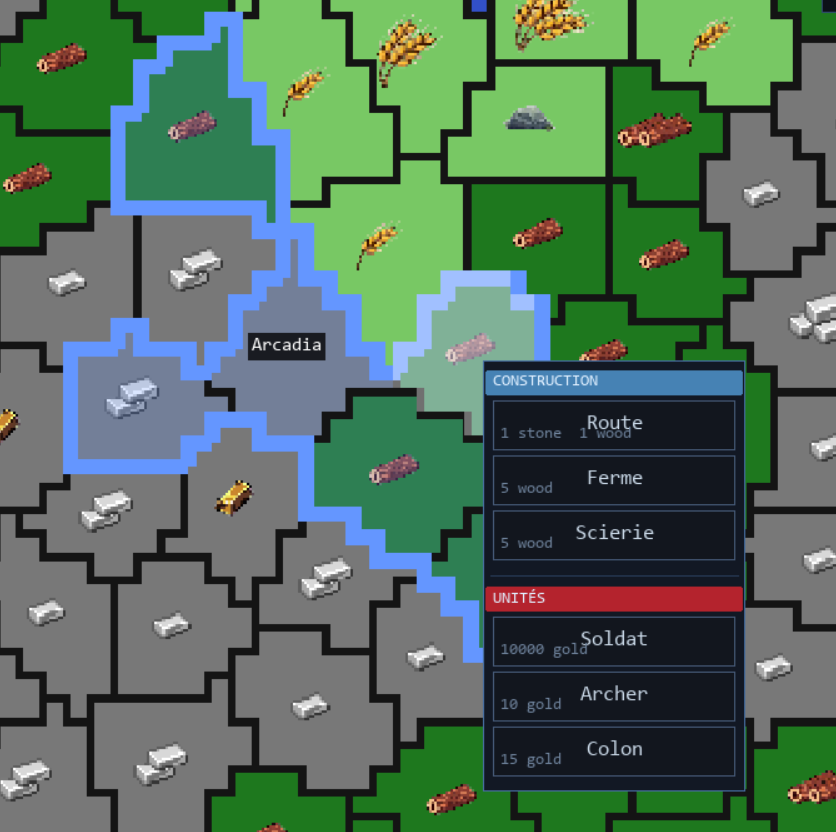
\includegraphics[width=0.55\textwidth]{../screenshots/fenetre_menu.png}
  \caption{Menu contextuel multi-catégories : Construction, Unités et Territoire}
  \label{fig:context_menu}
\end{figure}



\section{Description des méthodes importantes}
\label{sec:methodes}


\subsection{Génération de la carte : Map (world/map.py)}

La génération procédurale se déroule en sept étapes principales. On part d'une grille de cellules vierge qui sera
ensuite partitionnée en provinces (tuiles) et classifiée en biomes. On appelle $n$ le nombre de cellules de la grille
(environ 110 000 pour une carte de 444$\times$250 tuiles avec une taille ).

Par soucis de simplicités, certaines étapes sont regroupées dans une même section du fait de la
 similarité de leur but, mais elles sont programmées de manière distincte.

\subsubsection{Étape 1 : Échantillonnage de Poisson}
Les centres de provinces sont distribués uniformément sur la carte avec une contrainte de
distance minimale, en utilisant l'algorithme de Poisson Disk Sampling \cite{Ebeida2011-hx}. Une grille
d'accélération spatiale assure une complexité en $O(n)$.

\subsubsection{Étapes 2 et 3 : Attribution des biomes et partition de Voronoï}
Un bruit de Perlin multi-octaves génère une carte d'élévation. Des seuils distincts
classifient chaque cellule en biome (type de terrain) :
\begin{itemize}
    \item Eau : $n < -0{,}225$
    \item Plaine : $-0{,}225 \leq n < 0{,}14$
    \item Forêt : $0{,}14 \leq n < 0{,}325$
    \item Montagne : $n \geq 0{,}325$
    \item Désert : Plaine avec indice de chaleur élevé (second bruit indépendant)
\end{itemize}

Un KD-tree (\texttt{scipy.spatial.KDTree}) assigne chaque cellule de la grille à la province
la plus proche en $O(n \log n)$.

Puis chaque province obtient un biome majoritaire par vote de ses cellules, et une ressource est assignée
aléatoirement selon le biome qui a été attribué à la province en question.



\subsubsection{Étapes 4 et 5 : Nettoyage morphologique}
Un BFS détecte les composantes connexes et fusionne les micro-provinces sous un seuil de taille
minimum avec leurs voisines dominantes.

\subsubsection{Étapes 5 et 6 : Traitement des zones d'eau}
\begin{enumerate}
    \item Suppression des clusters d'eau isolés trop petits.
    \item Connexion des masses d'eau proches par des détroits.
    \item Élargissement des corridors d'eau trop fins.
    \item Fusion des tuiles d'eau en super-tuiles plus grandes (relaxation de Lloyd avec répulsion paramétrée par la distance au littoral).
\end{enumerate}

\subsubsection{Étape 7 : Graphe de voisinage et validation}
Construction du graphe à 8-connexité entre tuiles adjacentes, puis validation de l'intégrité
de la carte (cohérence bidirectionnelle entre cellules et tuiles).

\begin{figure}[H]
  \centering
  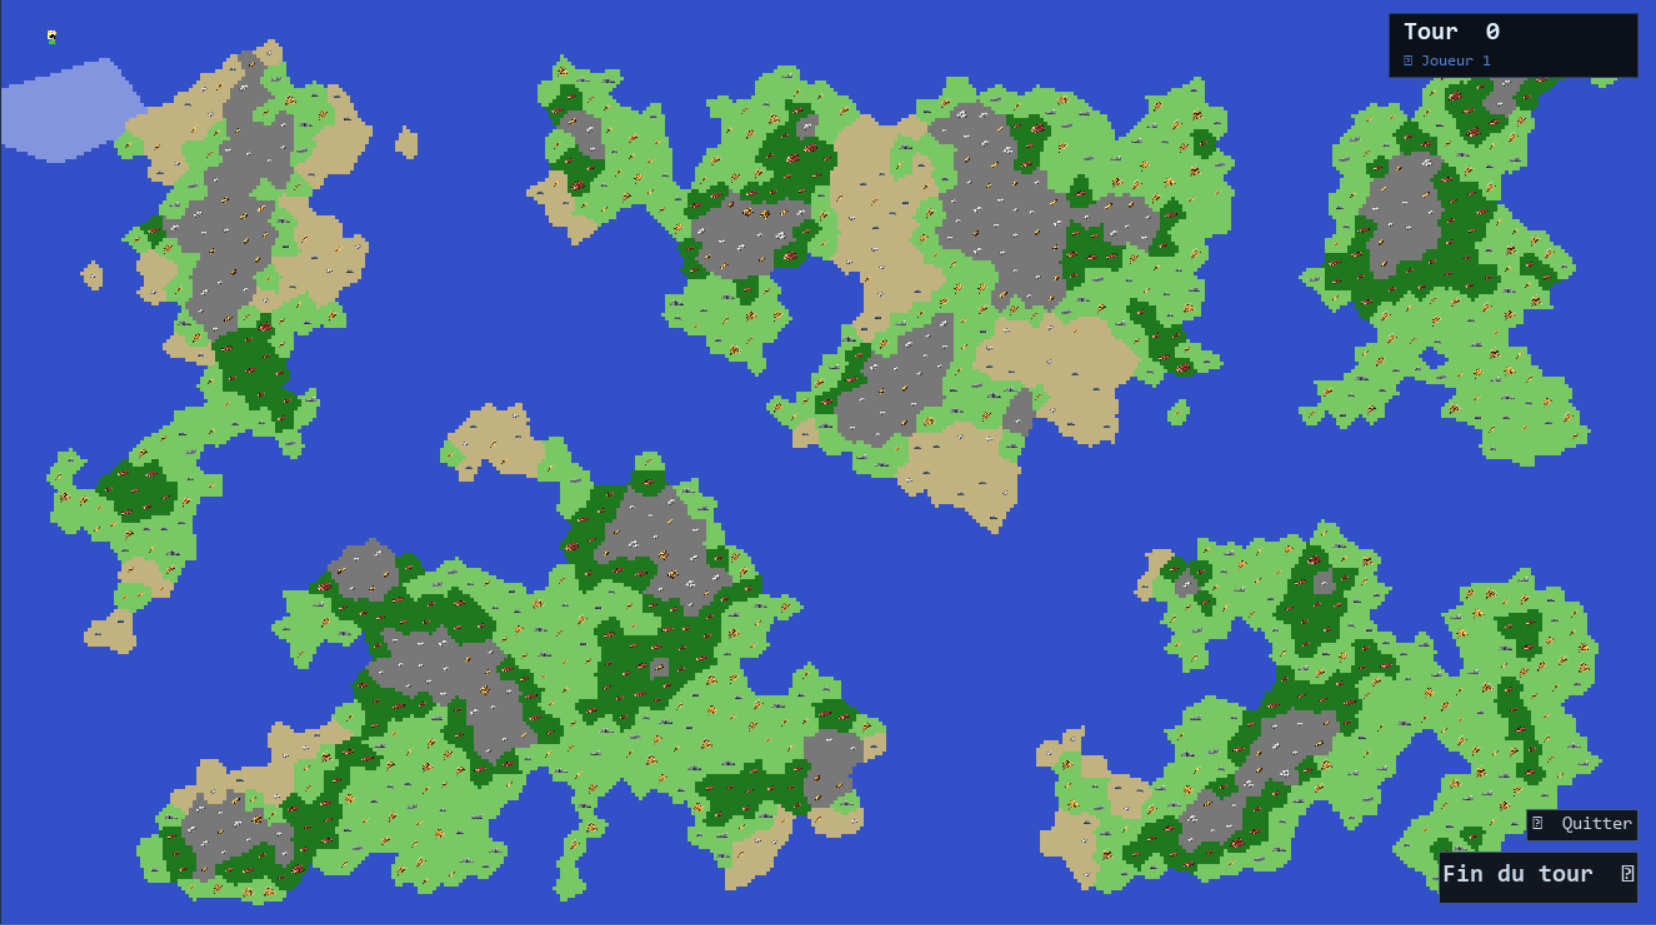
\includegraphics[width=0.85\textwidth]{../screenshots/génération de base.png}
  \caption{Exemple de carte générée procéduralement avec le pipeline Poisson--Voronoï--Perlin (plaine verte, forêt sombre, montagne grise, désert beige, eau bleue)}
  \label{fig:carte_generee}
\end{figure}

\subsection{Dijkstra : Movement.dijkstra\_reachable}

\begin{lstlisting}[style=python, caption={Algorithme de Dijkstra pour le déplacement}]
@staticmethod
def dijkstra_reachable(map_, start_tile_id, max_movement, unit_type):
    heap = [(0, start_tile_id)]
    distances = {start_tile_id: 0}
    visited = set()

    while heap:
        current_cost, current_tile_id = heapq.heappop(heap)
        if current_tile_id in visited:
            continue
        visited.add(current_tile_id)
        if current_cost > max_movement:
            continue

        for neighbor_tile_id in map_.tiles[current_tile_id].neighbors:
            if neighbor_tile_id in visited:
                continue
            terrain_cost = Movement.get_movement_cost(
                map_.tiles[neighbor_tile_id].biome, unit_type
            )
            if terrain_cost == float("inf"):
                continue
            new_cost = current_cost + terrain_cost
            if neighbor_tile_id not in distances or new_cost < distances[neighbor_tile_id]:
                distances[neighbor_tile_id] = new_cost
                heapq.heappush(heap, (new_cost, neighbor_tile_id))

    return distances
\end{lstlisting}

Les coûts de terrain varient selon le biome (1,0 en plaine, 1,5 en forêt, 2,0 en montagne,
$+\infty$ sur l'eau pour les unités terrestres) et sont modulés par des coefficients propres
à chaque type d'unité. Les unités avec \texttt{FLY=True} (Avion) ignorent ces coûts et se
déplacent librement sur toute la carte.

\subsection{Résolution du combat : Combat.compute\_damage}

La formule de dégâts intègre quatre facteurs :
\begin{equation}
    \text{dégâts} = (\text{ATK} - \text{DEF} \times m_\text{terrain}) \times m_\text{type} \times \frac{\text{PV}_\text{courant}}{\text{PV}_\text{max}}
\end{equation}
\begin{itemize}
    \item $m_\text{terrain}$ : modificateur de défense selon le biome du défenseur
    (montagne $\times 1{,}5$, forêt $\times 1{,}3$, plaine $\times 1{,}0$,
    désert $\times 0{,}9$, eau $\times 0{,}8$) ;
    \item $m_\text{type}$ : modificateur d'efficacité selon le triangle
    Soldat\,$\succ$\,Cavalerie\,$\succ$\,Archer\,$\succ$\,Soldat
    (valeurs 1,5 / 0,7) ;
    \item le ratio PV modélise l'affaiblissement d'une unité blessée.
\end{itemize}

La mécanique de \textbf{dash} de la cavalerie (attribut \texttt{DASH=True}) permet d'enchaîner
un déplacement et une attaque en un seul tour. L'attribut \texttt{ESCAPE=True} lui permet en
outre de se repositionner après avoir attaqué (sans avoir encore bougé).

\subsection{Expansion des villes : City.expend\_territory}

L'expansion utilise un BFS depuis la tuile centrale, limité au rayon \texttt{CITY\_EXTENSION\_RADIUS} (3 tuiles). Parmi les tuiles candidates libres (non-eau, non déjà attribuées), une tuile est tirée aléatoirement avec une probabilité inversement proportionnelle à sa distance :
\begin{equation}
    P(\text{tuile}_i) = \frac{1/d_i}{\displaystyle\sum_j 1/d_j}
\end{equation}
L'expansion n'est déclenchée que lors des tours où l'âge de la ville concernée appartient à la suite $[3, 5, 8, 13, 21, 34, 53, 89]$.

\subsection{Cycle de tour : GameEngine.end\_turn}

Le cycle complet d'un tour comporte trois phases :

\begin{enumerate}
    \item \textbf{Tour joueur} (\texttt{PLAYER\_TURN}) : le joueur humain interagit jusqu'à
    appuyer sur \og Fin du tour \fg{} (bouton ou touche Espace) ;
    \item \textbf{Tours IA} (\texttt{AI\_TURN}) : chaque royaume IA enregistré via
    \texttt{register\_ai()} joue son tour en appelant \texttt{ai.play\_turn(state, engine)}.
    Pendant cette phase, \texttt{input\_locked} est \texttt{True} et tous les événements
    clavier/souris joueur sont ignorés ;
    \item \textbf{Fin de tour} : mise à jour de l'économie (\texttt{Economy.update}),
    réinitialisation des drapeaux \texttt{has\_moved}/\texttt{has\_attacked}, vieillissement
    des villes et expansion éventuelle, recalcul du brouillard de guerre.
\end{enumerate}

\subsection{Fondation d'une ville : GameEngine.found\_city}

Un colon positionné sur une tuile terrestre libre peut fonder une ville via un clic droit.
La méthode vérifie les préconditions (type d'unité, existence de la tuile, absence de ville
existante, biome non-eau), crée l'objet \texttt{City}, calcule sa production initiale, puis
supprime le colon. Le nom de la ville est choisi aléatoirement dans une liste de noms
prédéfinis, sans réutiliser les noms déjà pris par le même joueur.

\subsection{Placement initial : GameEngine.setup\_start\_units}

À l'initialisation, chaque royaume reçoit un colon de départ positionné dans un coin de la
carte selon l'ordre d'inscription : coin haut-gauche, bas-droite, haut-droite, bas-gauche.
La méthode \texttt{get\_corner\_tile()} identifie la tuile non occupée la plus proche du coin
demandé en triant les tuiles par somme/différence de coordonnées.

\subsection{Bruit de Perlin : utils/noise.py}

Implémentation du bruit de Perlin standard avec table de permutation de Ken Perlin,
courbe de lissage quintic $f(t) = 6t^5 - 15t^4 + 10t^3$, et génération de bruit fractionnaire
Brownien (fBm) par superposition d'octaves :
\begin{equation}
    \text{fBm}(x, y) = \sum_{k=0}^{n-1} p^k \cdot \text{Perlin}\!\left(l^k \cdot x,\; l^k \cdot y\right)
\end{equation}
où $p$ est la persistance et $l$ la lacunarité. L'implémentation est une copie de la librairie \verb|noise|\cite{duncan_noise} disponible avec \verb|pip| mais non mise à jour depuis plusieurs années.



\section{Description des tests et des résultats}


\subsection{Stratégie de test}

Le projet dispose d'une suite de \textbf{334 tests unitaires automatisés} exécutés avec
\texttt{pytest}, organisés dans le dossier \texttt{test/}. Ces tests couvrent l'ensemble
des modules fonctionnels : modèle du monde, systèmes de jeu et utilitaires.

\subsubsection{Architecture de la suite de tests}

La suite est structurée en miroir de l'architecture du projet :

\begin{description}[leftmargin=2em]
    \item[\texttt{test/world/}] — Couche modèle (6 fichiers, $\approx 200$ tests) :
    \begin{itemize}
        \item \texttt{test\_tile.py} : initialisation, centre de gravité, \texttt{is\_water()},
        ajout/suppression/itération d'unités, \texttt{clear\_units()}, \texttt{\_\_repr\_\_} ;
        \item \texttt{test\_unit.py} : statistiques de toutes les classes d'unités (Soldat,
        Cavalerie, Archer, Colon, Bébé, Avion, Bateau), compteur d'ID global,
        \texttt{can\_move()}, \texttt{reset\_turn()}, masque de visibilité, fabrique
        \texttt{UNIT\_CLASS\_MAP} ;
        \item \texttt{test\_construction.py} : bonus de production des bâtiments (Ferme, Mine,
        Scierie, Route) pour chaque niveau de ressource (1 à 3) ;
        \item \texttt{test\_city.py} : auto-incrément d'ID, calcul de production par type
        de ressource, masque de visibilité, protection de la tuile centrale ;
        \item \texttt{test\_kingdom.py} : dataclass Kingdom, valeurs par défaut, \texttt{\_\_repr\_\_} ;
        \item \texttt{test\_resources.py} : énumération Resource, 16 membres, extraction du
        niveau (chiffres 1–3).
    \end{itemize}
    \item[\texttt{test/core/}] — Systèmes de jeu (4 fichiers, $\approx 120$ tests) :
    \begin{itemize}
        \item \texttt{test\_game\_state.py} : royaumes, villes, phases de tour, accumulation
        du bitmask de visibilité (avec patch de \texttt{core.game\_state.Map}) ;
        \item \texttt{test\_movement.py} : coûts de déplacement par biome/unité, distances
        Dijkstra, tuiles accessibles, tuiles attaquables, \texttt{execute\_move()},
        coût vers une tuile cible ;
        \item \texttt{test\_combat.py} : table d'efficacité (triangle Soldat/Cavalerie/Archer),
        calcul des dégâts (terrain, type, ratio PV), \texttt{can\_attack()}, \texttt{resolve()},
        \texttt{execute\_attack()} ;
        \item \texttt{test\_economy.py} : accumulation de la production de villes, déduction
        de l'entretien des unités pour le joueur actif uniquement ;
        \item \texttt{test\_visibility.py} : application du masque de brouillard de guerre.
    \end{itemize}
    \item[\texttt{test/utils/}] — Utilitaires (1 fichier, $\approx 25$ tests) :
    \begin{itemize}
        \item \texttt{test\_noise.py} : interpolation linéaire, gradient 2D, plage du bruit de
        Perlin (borné en $[-1, 1]$), déterminisme, octaves multiples, table de permutation.
    \end{itemize}
\end{description}

\subsubsection{Défis techniques et solutions}

\paragraph{Isolation de Pygame.}
Le module \texttt{world/unit.py} appelle \texttt{pygame.init()} et
\texttt{pygame.font.Sys\\Font()} à l'import, ce qui provoque une erreur dans un environnement
sans affichage. La solution adoptée est d'injecter un \texttt{MagicMock} dans
\texttt{sys.modules["pygame"]} \emph{avant} tout import de module projet, dans
\texttt{test/conftest.py}. Ceci garantit que tous les tests s'exécutent sans interface
graphique.

\paragraph{Substituts légers (MockMap, MockGameState).}
Les systèmes de jeu (Mouvement, Combat, Économie) opèrent sur un objet \texttt{GameState}
contenant une vraie \texttt{Map} générée procéduralement, ce qui rendrait les tests lents et
non déterministes. On leur substitue :
\begin{itemize}
    \item \texttt{MockMap} : dictionnaire de tuiles créées à la main avec voisinage explicite ;
    \item \texttt{MockGameState} : état minimal avec ressources, joueur courant et bitmask
    de visibilité pré-initialisés.
\end{itemize}
Cette approche réduit le temps d'exécution de la suite complète à moins de $0{,}2$\,s.

\paragraph{Compteurs globaux.}
\texttt{Unit.\_unit\_counter} et \texttt{City.\_next\_id} sont des attributs de classe
(entiers auto-incrémentés). Une fixture \texttt{autouse=True} dans \texttt{conftest.py}
les remet à zéro avant chaque test, garantissant l'isolation inter-tests.

\paragraph{Chemin relatif dans noise.py.}
\texttt{utils/noise.py} ouvre \texttt{"utils/perm.json"} avec un chemin relatif au
répertoire courant. Le conftest effectue \texttt{os.chdir(PROJECT\_ROOT)} au démarrage de
pytest pour que ce chemin soit toujours résolu correctement.


\subsubsection{Lancement de la suite}

\begin{myverbatim}[title={Commande de lancement des tests}]
# Depuis la racine du projet
python3 -m pytest test/

# Avec rapport de couverture détaillé
python3 -m pytest test/ -v --tb=short
\end{myverbatim}

\subsubsection{Tests manuels complémentaires}

En parallèle des tests automatisés, une méthode de validation de bout en bout reste
indispensable : lancer une partie, observer le comportement de chaque mécanique
(déplacement, combat, fondation de villes, économie) et vérifier visuellement la cohérence.
Les retours de débogage sont imprimés dans la console (\texttt{print}).

Un outil dédié, \texttt{perlin\_visualizer.py}, permet de visualiser interactivement le
bruit de Perlin et d'ajuster ses paramètres. La touche \textbf{R} régénère la carte en
temps réel, ce qui a facilité l'itération sur les paramètres de génération.

\subsection{Résultats obtenus}

\subsubsection{Génération de carte}

La génération procédurale produit des cartes cohérentes avec :
\begin{itemize}
    \item une distribution réaliste des biomes (plaines, forêts, montagnes, déserts, océans) ;
    \item des provinces de taille homogène (cible : $\approx 35$ cellules) ;
    \item des masses d'eau connectées entre elles via des détroits ;
    \item des ressources distribuées selon le biome (bois uniquement en forêt, fer/or en montagne, etc.).
\end{itemize}

\subsubsection{Mécaniques de jeu}

\begin{itemize}
    \item \textbf{Déplacement} : le pathfinding Dijkstra fonctionne correctement. La surbrillance
    des tuiles accessibles (bleue) est cohérente avec les points de mouvement et les coûts de terrain.
    \item \textbf{Combat} : la formule de dégâts est fonctionnelle. Le triangle d'efficacité
    (Soldat\,$\succ$\,Cavalerie\,$\succ$\,\\Archer\,$\succ$\,Soldat) est respecté. Le dash de la
    cavalerie fonctionne.
    \item \textbf{Économie} : la production des villes est calculée chaque tour. L'entretien
    des unités est déduit. Une balance négative en or n'est pas encore pénalisée.
    \item \textbf{Visibilité} : le brouillard de guerre (FoW) et la \textit{terra incognita} (TI)
    fonctionnent correctement. Le bitmask est suffisant pour la carte de démonstration. Les
    unités SCOUT (Archer, Avion) étendent la visibilité à 2 couronnes.
    \item \textbf{Fondation de villes} : un colon peut fonder une ville. L'expansion territoriale
    se déclenche aux bons tours et sélectionne aléatoirement une tuile voisine selon une loi de
    probabilité inverse à la distance.
    \item \textbf{Construction} : les bâtiments (Ferme, Mine, Route, Scierie) peuvent être
    construits depuis le menu contextuel si le joueur dispose des ressources nécessaires.
    \item \textbf{Achat de tuile} : une tuile neutre adjacente à une ville peut être annexée
    pour 10 pièces d'or via le menu contextuel (catégorie Territoire).
    \item \textbf{Achat d'unité} : un Soldat, Archer ou Colon peut être acheté directement
    depuis le menu contextuel sur les tuiles d'une ville du joueur.
\end{itemize}

\subsubsection{Interface graphique}

L'IHM est fonctionnelle :
\begin{itemize}
    \item panoramique fluide à la souris et au clavier (Z/S/Q/D) ;
    \item zoom de 1$\times$ à 25$\times$ centré sur la position du curseur ;
    \item barre latérale affichant les ressources et les boutons d'action avec animations lissées ;
    \item barre de statut affichant les informations de la tuile survolée (biome, ressource, constructions, unité) ;
    \item indicateur de tour animé (pulsation bleue en tour joueur, pulsation rouge en tour IA) ;
    \item rendu optimisé par mise en cache des surfaces \texttt{Pygame} (reconstruction uniquement
    si l'état a changé).
\end{itemize}

\begin{figure}[H]
  \centering
  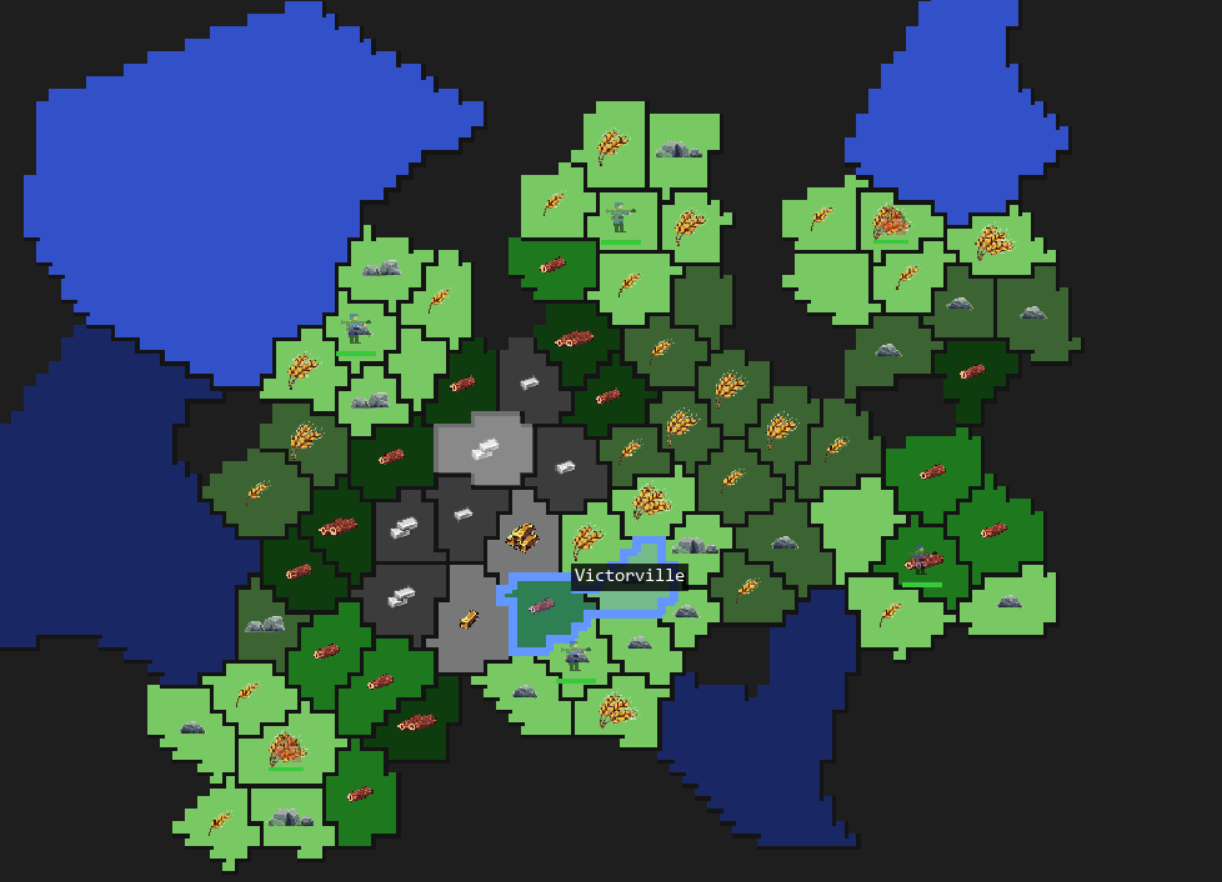
\includegraphics[width=0.85\textwidth]{../screenshots/FOW_TI.png}
  \caption{Rendu du brouillard de guerre (\textit{Fog of War}) et de la \textit{Terra Incognita} : zones noires (inconnues), grises (déjà explorées), claires (actuellement visibles)}
  \label{fig:fog_of_war}
\end{figure}



\section{Conclusion}

Le projet \textbf{Imperium Novum } remplit ses objectifs principaux : il constitue un jeu 4X
simplifié, jouable et structuré, avec une architecture orientée objet modulaire et une interface
graphique interactive. Les quatre axes du genre (exploration, expansion, exploitation,
extermination) sont représentés, même si certains restent partiellement implémentés.

Les points forts du projet sont la qualité du pipeline de génération procédurale de carte
(Poisson + Voronoï + Perlin + post-traitements hydrographiques), le système de déplacement
basé sur Dijkstra, et l'architecture en systèmes découplés coordonnés par le moteur. Le
cadre multi-royaumes et l'interface abstraite \texttt{BaseAI} constituent une base solide
pour l'ajout d'adversaires automatiques sans modifier le code existant.

Ce projet nous a surtout permis de réaliser qu'il existe un monde entre \textit{coder} et
\textit{créer un jeu}. Fixer un coût d'entretien à une unité tient en une ligne de code ;
équilibrer ce coût pour que la partie soit intéressante du début à la fin est un problème
d'une toute autre nature. Il en va de même pour les conditions de victoire : écrire
\texttt{if gold > 10000} est trivial, mais concevoir une fin de partie cohérente, qui ne
lasse pas le joueur et qui reste ouverte jusqu'au bout, relève de la conception de jeu bien
plus que de l'informatique.

L'implémentation d'une IA adversaire illustre encore mieux ce fossé. Le défi ne venait pas
du code, l'interface \texttt{BaseAI} est en place, mais du fait que nous sommes les
concepteurs du jeu et savons donc, par définition, comment y jouer parfaitement. Vouloir
inculquer des stratégies à une IA sans passer par de l'apprentissage automatique revient
à écrire à la main tout ce que nous faisons intuitivement, ce qui constituerait à lui seul
un projet informatique entier.

Il faut également souligner que la génération procédurale de la carte est d'une complexité
algorithmique telle qu'elle constitue elle aussi un projet à part entière. Le pipeline
Poisson--Voronoï--Perlin, les post-traitements hydrographiques et les heuristiques de
validation ont mobilisé plus de \textbf{30 heures de travail} à eux seuls.

Ce projet nous a confortés dans notre capacité à concevoir, maintenir et faire évoluer une
base de code conséquente et multi-couches. Il nous a surtout fait prendre conscience que le
développement va bien au-delà du terminal : le retour utilisateur est primordial, et c'est
ce que les tests illustrent parfaitement. Une batterie de 334 tests ne peut pas reproduire
les centaines d'actions imprévues qu'une vraie base de joueurs découvrirait en quelques
heures de partie, deux bugs non trouvé jusqu'à lors ont pourtant été détectés à leur rédaction. Cela confirme
que formaliser les tests est bénéfique dès maintenant.

En définitive, la réalisation de ce projet s'est révélée particulièrement formatrice.
Au-delà des compétences techniques acquises, cette expérience nous apporte aujourd'hui le recul
méthodologique et la maturité nécessaires pour appréhender la suite de notre parcours avec une
réelle sérénité. Nous sommes désormais pleinement armés pour identifier et privilégier les choix
 d'avenir qui correspondent le mieux à nos aspirations professionnelles.



\newpage

% affiche la bibliographie (si utilisée)
\printbibliography

\newpage

% ============================================================
\section*{Annexes}
\addcontentsline{toc}{section}{Annexes}
% ============================================================

% -----------------------------------------------------------
\subsection*{A – Arbre des fichiers du projet}
\addcontentsline{toc}{subsection}{A – Arbre des fichiers du projet}
% -----------------------------------------------------------

\begin{myverbatim}
proj_info/
|-- run_project.py          # point d'entree
|-- config.py               # constantes globales (GameConfig)
|-- core/
|   |-- game_engine.py      # facade principale
|   |-- game_state.py       # etat mutable (GameState, TurnPhase)
|   |-- ai/
|   |   |-- base_ai.py      # interface abstraite BaseAI
|   |   |-- simple_ai.py    # implementation IA simple
|   |-- systems/
|       |-- combat.py
|       |-- economy.py
|       |-- movement.py
|       |-- visibility.py
|-- ui/
|   |-- main.py             # boucle principale pygame
|   |-- ui_manager.py       # rendu & menu contextuel
|   |-- sidebar.py
|-- utils/
|   |-- noise.py            # bruit de Perlin
|   |-- perm.json           # table de permutation de Ken Perlin
|-- world/
    |-- biome.py            # enum Biome
    |-- city.py             # classe City
    |-- construction.py     # Farm, Mine, Scierie, Road
    |-- kingdom.py          # dataclass Kingdom
    |-- map.py              # generation de carte (Map)
    |-- resources.py        # enum Resource
    |-- selector.py         # UnitSelector
    |-- tile.py             # classe Tile (province)
    |-- unit.py             # Unit + sous-classes + UNIT_CLASS_MAP
\end{myverbatim}

% -----------------------------------------------------------
\subsection*{B – Fichier \texttt{config.py} complet}
\addcontentsline{toc}{subsection}{B – Fichier config.py complet}
% -----------------------------------------------------------

\begin{lstlisting}[style=python, caption={Fichier \texttt{config.py} – constantes globales}, label={lst:config_full}]
class GameConfig:
    # --- Carte ---
    TILE_SIZE = 2           # pixels par cellule de grille
    TILE_AVG_AREA = 35      # surface moyenne d'une tuile Voronoi
    HEIGHT = 250
    WIDTH = (HEIGHT * 16) // 9

    FPS = 60

    SCREEN_WIDTH  = WIDTH  * TILE_SIZE
    SCREEN_HEIGHT = HEIGHT * TILE_SIZE

    # --- Generation de la carte ---
    LOG_MAP_GENERATION    = True
    BORDER_STRENGTH       = 2.75
    OCEANIC_COEFF         = 1.5    # plus eleve = moins d'eau
    OCEANIC_OFFSET        = 0.1
    DESERT_HEAT_THRESHOLD = 0.15
    MIN_WATER_CLUSTER_SIZE  = 2    # clusters <= 2 tuiles convertis en terre
    WATER_CONNECT_MIN_SIZE  = 8    # taille min d'une masse d'eau a relier
    WATER_BRIDGE_MAX_HOPS   = 3    # distance max pour relier deux masses d'eau
    WATER_TILE_SIZE_COEFF   = 8    # fusion de tuiles d'eau proches

    # --- Couleurs des biomes (R, G, B) ---
    BIOME_COLORS = {
        Biome.BLANK:    (  0,   0,   0),
        Biome.WATER:    ( 50,  80, 200),
        Biome.PLAIN:    (120, 200, 100),
        Biome.FOREST:   ( 30, 120,  30),
        Biome.MOUNTAIN: (120, 120, 120),
        Biome.DESERT:   (194, 178, 128),
    }

    # --- Interface ---
    SIDEBAR_WIDTH            = 210  # largeur barre laterale gauche
    STATUS_H                 = 52   # hauteur barre de statut bas
    CONSTRUCTION_MENU_WIDTH  = 200
    CONSTRUCTION_MENU_ITEM_H = 40
    CONSTRUCTION_MENU_PADDING= 10

    # --- Ressources ---
    RESOURCE_BASE_SCALE = 3

    # --- Villes ---
    CITY_MIN_TURN_EXTENTION_AVAILABLE = [3, 5, 8, 13, 21, 34, 53, 89]
    CITY_EXTENSION_RADIUS             = 3    # distance max fondatrice -> nouvelle province
    CITY_EXTENSION_FOOD_POP_MIN_RATION= 1.25 # ration min nourriture/habitant
\end{lstlisting}

% -----------------------------------------------------------
\subsection*{C – Biomes, coûts de déplacement et modificateurs de combat}
\addcontentsline{toc}{subsection}{C – Biomes, coûts et modificateurs}
% -----------------------------------------------------------

Le tableau suivant synthétise les propriétés de chaque biome telles que définies dans
\texttt{core/systems/}\texttt{movement.py} et \texttt{core/systems/combat.py}.

\begin{table}[H]
\centering
\caption{Propriétés des biomes}
\label{tab:biomes}
\renewcommand{\arraystretch}{1.3}
\begin{tabular}{|l|c|c|c|}
\hline
\textbf{Biome} & \textbf{Coût de déplacement (base)} & \textbf{Modificateur défense} & \textbf{Couleur (RGB)} \\
\hline
Plaine   & 1,0  & $\times 1{,}0$ (neutre)    & (120, 200, 100) \\
Forêt    & 1,5  & $\times 1{,}3$ (+30\,\%)   & (30, 120, 30)   \\
Montagne & 2,0  & $\times 1{,}5$ (+50\,\%)   & (120, 120, 120) \\
Désert   & 1,2  & $\times 0{,}9$ ($-10$\,\%) & (194, 178, 128) \\
Eau      & $\infty$ (infranchissable) & $\times 0{,}8$ ($-20$\,\%) & (50, 80, 200) \\
\hline
\end{tabular}
\end{table}

Les modificateurs de déplacement s'appliquent \emph{à la place} du coût de base pour
les unités qui possèdent un modificateur explicite :

\begin{table}[H]
\centering
\caption{Modificateurs de déplacement par type d'unité}
\label{tab:movement_modifiers}
\renewcommand{\arraystretch}{1.3}
\begin{tabular}{|l|c|c|c|c|c|}
\hline
\textbf{Unité} & \textbf{Plaine} & \textbf{Forêt} & \textbf{Montagne} & \textbf{Désert} & \textbf{Eau} \\
\hline
Soldat   & 1,0 & 1,5 & 2,0       & 1,2 & $\infty$ \\
Archer   & 1,0 & 1,5 & 2,0       & 1,2 & $\infty$ \\
Cavalerie & \textbf{0,8} & \textbf{1,8} & \textbf{2,5} & 1,2 & $\infty$ \\
Colon    & 1,0 & \textbf{1,0} & \textbf{1,0} & \textbf{1,0} & \textbf{1,0} \\
Avion    & 1,0 & \textbf{1,0} & \textbf{1,0} & \textbf{1,0} & \textbf{1,0} \\
Bateau   & 1,0 & \textbf{1,0} & \textbf{1,0} & \textbf{1,0} & \textbf{1,0} \\
\hline
\end{tabular}
\end{table}
\noindent Les valeurs en gras indiquent un écart par rapport au coût de base du biome.

% -----------------------------------------------------------
\subsection*{D – Ressources, constructions et productions}
\addcontentsline{toc}{subsection}{D – Ressources, constructions et productions}
% -----------------------------------------------------------

\paragraph{Types de ressources.}
Chaque tuile peut porter une ressource parmi trois niveaux (1, 2, 3) :
\texttt{GOLD}, \texttt{FOOD}, \texttt{WOOD}, \texttt{IRON}, \texttt{STONE} (plus \texttt{NONE}).
Le niveau détermine le multiplicateur de production de la construction associée.

\begin{table}[H]
\centering
\caption{Constructions : coûts et bonus de production}
\label{tab:constructions}
\renewcommand{\arraystretch}{1.3}
\begin{tabular}{|l|l|l|p{6cm}|}
\hline
\textbf{Construction} & \textbf{Coût} & \textbf{Ressource cible} & \textbf{Bonus produit} \\
\hline
Ferme    & 5 bois & \texttt{FOOD\textit{n}} & \texttt{food += n} (ou +1 par défaut) \\
Scierie  & 5 bois & \texttt{WOOD\textit{n}} & \texttt{wood += n} (ou +1 par défaut) \\
Mine     & 2 pierre + 3 bois & \texttt{IRON\textit{n}} / \texttt{GOLD\textit{n}} / \texttt{STONE\textit{n}} &
    \texttt{iron += n}, \texttt{stone += 1} \quad ou\quad
    \texttt{gold += n}, \texttt{stone += 1} \quad ou\quad
    \texttt{stone += n} \\
Route    & 1 pierre + 1 bois & – & \texttt{movement bonus = 1} (réduction du coût de passage) \\
\hline
\end{tabular}
\end{table}

\noindent Une tuile peut accueillir au maximum \textbf{une route} et \textbf{un bâtiment} simultanément.

% -----------------------------------------------------------
\subsection*{E – Algorithme de bruit de Perlin (\texttt{utils/noise.py})}
\addcontentsline{toc}{subsection}{E – Algorithme de bruit de Perlin}
% -----------------------------------------------------------

L'implémentation est extraite et simplifiée depuis la bibliothèque \texttt{noise}
(non maintenue depuis 2018), en ne conservant que la partie 2D nécessaire à la génération
de carte.

\paragraph{Principe général.}
Le bruit de Perlin génère une valeur continue en $[-1, 1]$ pour tout point $(x, y)$
du plan réel. Le résultat est \emph{pseudo-aléatoire} mais \emph{cohérent spatialement}
(les points proches ont des valeurs proches), ce qui produit des formes organiques.

\paragraph{Étapes de calcul (\texttt{\_noise(x, y)}).}
\begin{enumerate}
    \item \textbf{Localisation de cellule.} On identifie la cellule entière
          $\lfloor x \rfloor$, $\lfloor y \rfloor$ contenant le point, puis on
          calcule les coordonnées relatives $x' = x - \lfloor x \rfloor \in [0,1]$
          et $y' = y - \lfloor y \rfloor \in [0,1]$.
    \item \textbf{Courbe d'atténuation (quintic).} Pour éviter les discontinuités
          visibles, les coordonnées relatives sont lissées par la courbe de Ken Perlin :
          \[
            f(t) = 6t^5 - 15t^4 + 10t^3
          \]
    \item \textbf{Vecteurs de gradient.} Les 4 coins de la cellule sont hachés via
          la table de permutation \texttt{PERM[512]} (table standard de Ken Perlin,
          doublée pour éviter les débordements d'indice). Chaque hash est converti
          en l'un des 8 vecteurs de gradient 2D.
    \item \textbf{Interpolation bilinéaire.} Les produits scalaires
          $\text{grad} \cdot (x', y')$ aux 4 coins sont interpolés avec les
          valeurs atténuées $f_x$ et $f_y$.
\end{enumerate}

\paragraph{Bruit fractal (\texttt{perlin\_noise}).}
Pour obtenir un terrain naturel, on superpose plusieurs couches (\emph{octaves}) :
\[
  \text{total} = \sum_{k=0}^{N-1} a_k \cdot \text{noise}\!\left(f_k x,\; f_k y\right),
  \quad
  f_k = \text{lacunarity}^k, \quad a_k = \text{persistence}^k
\]
Le résultat est normalisé par la somme des amplitudes $\sum a_k$.
La carte utilise plusieurs octaves pour superposer des détails fins sur la structure
globale des continents.

\begin{lstlisting}[style=python, caption={Signature de \texttt{perlin\_noise} (utils/noise.py)}, label={lst:perlin}]
def perlin_noise(x, y,
                 octaves=1,
                 persistence=0.5,   # amplitude diminue a chaque octave
                 lacunarity=2.0,    # frequence double a chaque octave
                 repeatx=1024, repeaty=1024,
                 base=0):
    ...
\end{lstlisting}

% -----------------------------------------------------------
\subsection*{F – Captures d'écran annotées}
\addcontentsline{toc}{subsection}{F – Captures d'écran annotées}
% -----------------------------------------------------------

\begin{figure}[H]
\centering
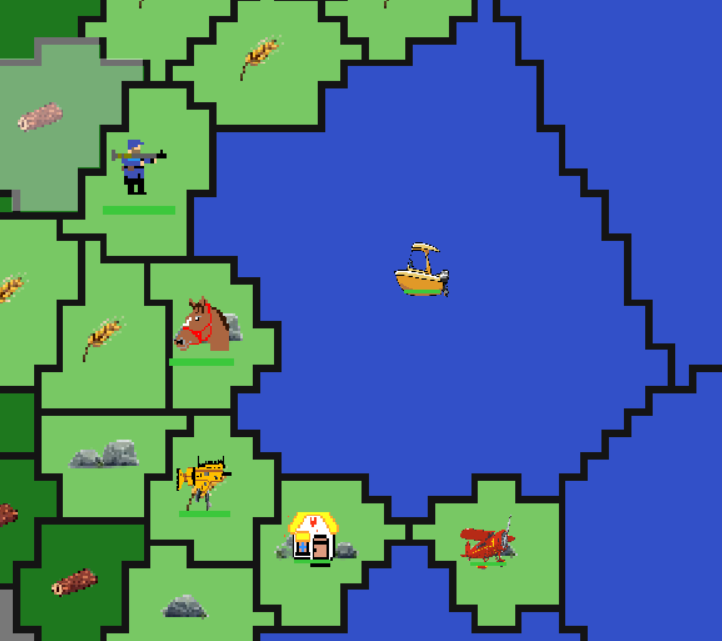
\includegraphics[width=0.85\textwidth]{../screenshots/unites.png}
\caption{Diversité des unités en jeu : soldat, cavalerie, avion, bateau (naviguant sur l'eau) et colon avec bâtiment}
\label{fig:annex_ihm}
\end{figure}

\begin{figure}[H]
\centering
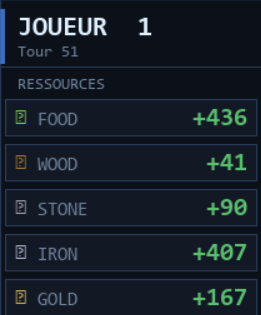
\includegraphics[width=0.45\textwidth]{../screenshots/ex_ressources.png}
\caption{Barre latérale : ressources du joueur 1 au tour 51 (nourriture, bois, pierre, fer, or)}
\label{fig:annex_sidebar}
\end{figure}

\end{document}

